\section{交流回路・共振と電磁波}

% ===========================================================================
%  再編（2026-09-24）：第4章 電磁気学 の第32回（電磁気学の最終回）．
%  原本の 第41回「振動回路・交流回路(2)」の全体（41.1 交流のベクトル表示／41.2 RLC の直列回路／
%  41.3 RLC 直列共振／41.4 複雑な交流回路／41.5 電磁波）に，電磁気の章末問題 [97][98] を加えた．
%
%  ・練習は12題．練習番号は第31回（［111］〜［119］）の続き．
%      ［120］＝㊶[85]（A問題：インピーダンス）  ［121］＝㊶[86]（A問題：電磁波）
%      ［122］＝㊶[87]（RL直列）  ［123］＝㊶[88]（RC直列）  ［124］＝㊶[89]（RLC直列共振・指定）
%      ［125］＝㊶[90]（グラフの読み取り）  ［126］＝㊶[91]（並列共振・指定）  ［127］＝㊶[92]（複雑な交流回路）
%      C問題 ［128］＝㊶[93]（直流・交流回路）  ［129］＝㊶[94]（電磁波の発生）
%            ［130］＝㊶章末[97]（コの字型回路）  ［131］＝㊶章末[98]（リサジュー図形）
%    A問題が2題あるが，［120］は交流回路，［121］は電磁波で内容が別なので統合しなかった．
%
%  ・例題は4題．原本の 例題43・44・45・46．第31回が【例題35】〜【例題39】なので
%    \setcounter{nombre}{39} として【例題40】〜【例題43】と表示される．
%
%  ・【重要】原本の講義編は Google Drive の OCR テキストしか取れなかったので，例題の問題文は
%    OCR から復元し，図は circuitikz で描き起こした（`mkfig_new32ex.py`）．要照合：
%      ・例題40〜42（原本43〜45）の設問は OCR の通り．電流を $I_0\sin(\omega t-\varphi)$ と置く形も OCR の通り．
%      ・例題43（原本46）：OCR からは「R, L, C を用いて図のような回路」「AD 間に 60 Hz の交流電源」
%        「C 点に対する B 点の電位 $V_{\mathrm{BC}}$ がグラフのように変化」「$R=120\,\mathrm{k\Omega}$，
%        $\omega L=60\,\mathrm{k\Omega}$，$\frac{1}{\omega C}=120\,\mathrm{k\Omega}$」「(1) $I_L(t)$，$I_C(t)$
%        （B→C を正）」「(2) $V_{\mathrm{AB}}$，$V_{\mathrm{AD}}$」しか読めない．
%        **回路（A–R–B，BC 間に L と C の並列，C–D は導線）とグラフの振幅 12 V は再構成**した．
%
%  ・原本の本文に無く，練習・例題が前提にしていたものを加筆した：
%      ・32.1 に{実効値でベクトル図を描いてもよい}（全体を $\frac{1}{\sqrt2}$ 倍しても角度は変わらない）．
%        練習［124］［127］の解答が実効値でベクトル図を描いている．
%      ・32.3 に{共振時の特徴}（$V_L$ と $V_C$ が打ち消し合い電源電圧がすべて抵抗にかかる，消費電力が最大）
%        と，{Q 値の考え方}の代わりに「$V_L$・$V_C$ は電源電圧より大きくなりうる」（練習［124］(3)(4)）．
%      ・32.4 に{並列共振}（LC 並列部の電流が打ち消し合い，電源から電流が流れない）と，
%        {周波数によるコイル・コンデンサーのふるまい}（練習［126］(2) の要）．
%      ・32.5 に{リサジュー図形}（練習［131］の前提．原本では解答の指針で初めて説明していた）．
%
%  ・原本（問題編の解答）の誤りを直した（いずれもコメントで明記）：
%      (a) 練習［123］(3) の解答「$\frac{6.0}{3\times 10^3}$」→ $30\times 10^3$（問題文は $30\,\mathrm{k\Omega}$．答の値は正しい）．
%      (b) 練習［128］の指針「コイルは容量リアクタンスを持つ」→ 誘導リアクタンス．
%      (c) 旧回の番号による参照（「B問題［34］と同様に」「テキスト例題を参照」）を付け替えた．
%
%  ・図：講義の図は講義編から切り出し済みのもの（img/text/text2_p88・p93）．
%    練習・解答の図は `mkfig_new32.py`＋`jobs_new32.py`，例題の図は `mkfig_new32ex.py`．
% ===========================================================================

% 例題番号：第31回が【例題35】〜【例題39】
\setcounter{nombre}{39}

\subsection{交流のベクトル表示}

\begin{zuright}{46mm}
\hspace{1zw}右図の回路で，時刻$t$の電源電圧を$V(t)$，抵抗にかかる電圧を$V_R(t)$，コイルにかかる電圧を$V_L(t)$とすると，キルヒホッフの第二法則より
\[V(t)=V_R(t)+V_L(t)\]
が成り立つ．
一般に，各素子の電圧は
\[V_R(t)=V_{R0}\sin(\omega t+\theta_1),\quad V_L(t)=V_{L0}\sin(\omega t+\theta_2)\]
のように位相の異なる三角関数になるので，そのまま足し算をするのは計算が煩雑になる．
\zusep

\includegraphics[keepaspectratio,width=44mm]{text2_p88_fig1.png}
\end{zuright}

\begin{zuright}{62mm}
\hspace{1zw}そこで右図のように，長さ$V_{R0}$，$x$軸からの角$\omega t+\theta_1$のベクトル$\overrightarrow{V_R}$を考えると，その$y$軸への投影が$V_R(t)$になる．同様に，長さ$V_{L0}$，角$\omega t+\theta_2$のベクトル$\overrightarrow{V_L}$の$y$軸への投影が$V_L(t)$になる．
すると，{\gtfamily $V_R(t)+V_L(t)$は2つのベクトルの和$\overrightarrow{V_R}+\overrightarrow{V_L}$の$y$軸への投影に等しい}．
三角関数の和を，図形的なベクトルの和に置き換えて考えることができるのである．
これを{\gtfamily 交流のベクトル表示}という．
ベクトル全体は角速度$\omega$で反時計回りに回転しているが，ベクトルどうしの角度（位相差）と長さは変わらないので，ある瞬間の図だけを描けばよい．
\zusep

\includegraphics[keepaspectratio,width=60mm]{text2_p88_fig2.png}
\end{zuright}

31.7 のまとめ枠をベクトルで言い直すと，電流ベクトルを基準にして
\begin{description}
\item[\MARU{1}] 抵抗の電圧ベクトルは，長さ$RI_0$で電流と{\gtfamily 同じ向き}
\item[\MARU{2}] コイルの電圧ベクトルは，長さ$\omega LI_0$で電流より{\gtfamily $90^\circ$進んだ向き}（反時計回りに$90^\circ$）
\item[\MARU{3}] コンデンサーの電圧ベクトルは，長さ$\dfrac{I_0}{\omega C}$で電流より{\gtfamily $90^\circ$遅れた向き}（時計回りに$90^\circ$）
\end{description}
となる．

なお，交流回路では各電圧・電流に位相差があるので，{\gtfamily 最大値や実効値を単純に足してキルヒホッフの第二法則を立ててはならない}．第二法則が成り立つのは瞬時値（ベクトルの和）についてだけである．
% 加筆：実効値でベクトル図を描いてよい（練習［124］［127］の解答が前提）．
また，ベクトル図全体を$\dfrac{1}{\sqrt{2}}$倍しても角度（位相差）は変わらないので，{\gtfamily ベクトルの長さを実効値にとって描いてもよい}．問題文が実効値で与えられているときはこの方が便利である．

\bsNeed{30mm}
\begin{matome}{交流のベクトル表示}
 \hspace{3mm} $y$軸への投影が瞬時値になるベクトルを考え，三角関数の和を\AnaB{ベクトルの和}で求める\\
 \hspace{3mm} 電流を基準に，抵抗は同じ向き，コイルは$90^\circ$進み，コンデンサーは$90^\circ$遅れ
\end{matome}

\subsection{抵抗・コイル・コンデンサーの直列回路}

ベクトル表示と各素子の電圧・電流の関係を使って，交流回路を流れる電流を求める．
交流回路をベクトル図で考えるときは，次の順序で考えるとよい．
\begin{description}
\item[\MARU{1}] 直列接続では{\gtfamily 電流が共通}なので，まず電流を仮定してベクトルで描く．
\item[\MARU{2}] 電流をもとに，各素子の電圧ベクトルを描く．
\item[\MARU{3}] 各素子の電圧ベクトルの和が，電源電圧のベクトルに等しいとおく（三平方の定理が使えることが多い）．
\end{description}

%%%%%%%%%%  例題40（原本の【例題43】）  %%%%%%%%%%%%%%%%%%%%
\bsNeed{60mm}
\begin{reidaiunit}
\begin{reidai}{RL直列回路}
\begin{zuright}{44mm}
\hspace{1zw}抵抗値$R\U{\Omega}$の抵抗と自己インダクタンス$L\U{H}$のコイルを，図のように角周波数$\omega\U{rad/s}$の交流電源に接続した．図の$-$側に対する$+$側の電圧の瞬時値が$V(t)=V_0\sin\omega t\U{V}$であるときに回路に流れる交流電流を求めたい．以下の問いに答えよ．
\zusep
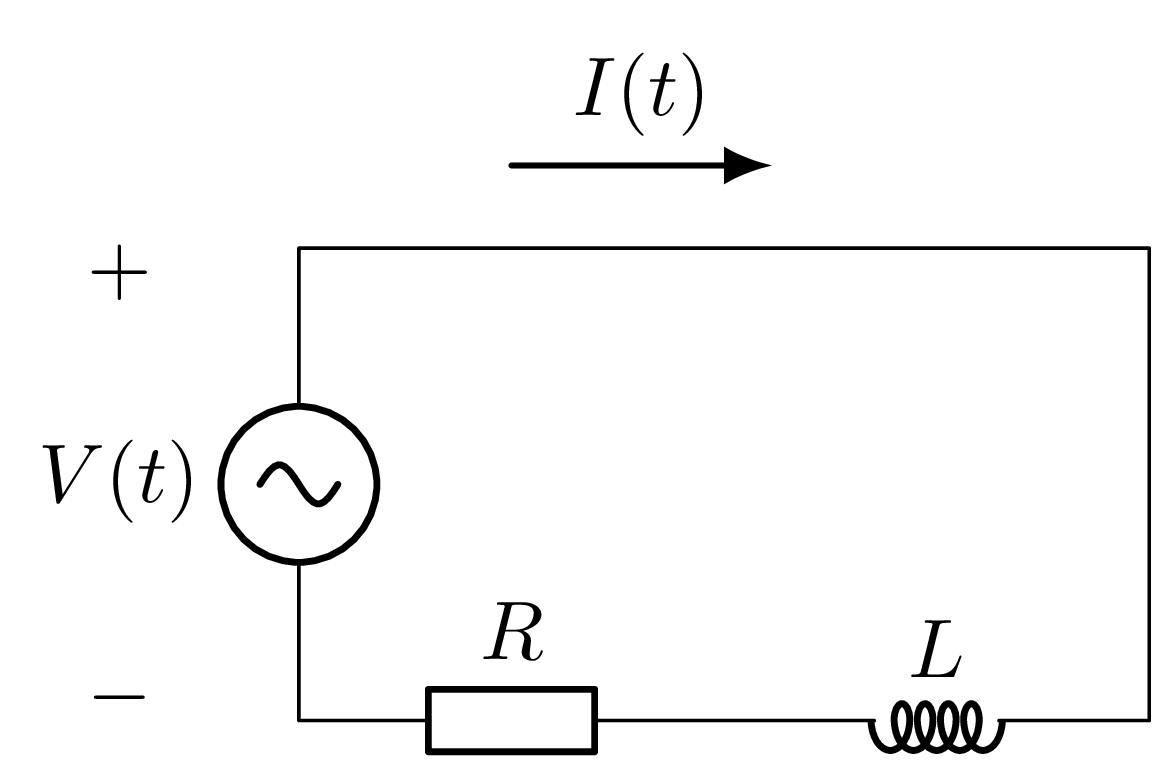
\includegraphics[keepaspectratio,width=40mm]{fig/n32_ex40_zu.png}
\end{zuright}
\begin{komon}
\ko{1} 交流電流は電源と同じ角周波数で変化すると考えられるので，流れている電流を$I(t)=I_0\sin(\omega t-\varphi)\U{A}$の形に仮定する．このとき，抵抗およびコイルにかかる電圧の瞬時値$V_R(t)$，$V_L(t)$を求めよ．
\ko{2} 電流をベクトルで表したとき，抵抗にかかる電圧ベクトル$\overrightarrow{V_R}$，コイルにかかる電圧ベクトル$\overrightarrow{V_L}$を図示せよ．
\ko{3} 電源電圧ベクトルを図示し，$V_0$および$\omega t$をそれぞれ図に記入せよ．
\ko{4} 以上を用いて，流れる交流電流の最大値$I_0\U{A}$を求めよ．
\ko{5} 電圧と電流の位相のずれの正接$\tan\varphi$を求めよ．
\end{komon}
\end{reidai}

\begin{sisinE}
直列接続なので電流が共通である．電流ベクトルをもとに，抵抗の電圧は同じ向き，コイルの電圧は$90^\circ$進んだ向きに描く．
2つの電圧ベクトルは直交するので，その和（電源電圧）の長さは三平方の定理で求まる．
\end{sisinE}

\Key{直列接続\ $\Rightarrow$\ 流れる電流$I(t)$が共通．電流ベクトルをもとにして電圧ベクトルを作図}

\begin{kaitou}
\begin{komon}
\ko{1} \[V_R(t)=RI_0\sin(\omega t-\varphi),\quad V_L(t)=\omega LI_0\sin\Bigl(\omega t-\varphi+\frac{\pi}{2}\Bigr)\Ans\]
\item[{\makebox[1.9zw][r]{(2)(3)}}] 次図のようになる．電源電圧ベクトルは$x$軸と角$\omega t$をなし，電流ベクトルより$\varphi$だけ進んでいる．\Ans
       \begin{center}\AnaFig{50mm}{fig/n32_ex40_ans.png}{fig/n32_ex40_ans.png}\end{center}
\ko{4} 三平方の定理より$V_0^2=(RI_0)^2+(\omega LI_0)^2$なので
       \Ana{I_0=\frac{V_0}{\sqrt{R^2+\omega^2L^2}}\U{A}\Ans}
\ko{5} \[\tan\varphi=\frac{\omega LI_0}{RI_0}=\frac{\omega L}{R}\Ans\]
       （電流の位相は電圧より$\varphi$だけ遅れている．）
\end{komon}
\end{kaitou}
\end{reidaiunit}

%%%%%%%%%%  例題41（原本の【例題44】）  %%%%%%%%%%%%%%%%%%%%
\bsNeed{60mm}
\begin{reidaiunit}
\begin{reidai}{RC直列回路}
\begin{zuright}{44mm}
\hspace{1zw}抵抗値$R\U{\Omega}$の抵抗と電気容量$C\U{F}$のコンデンサーを，図のように角周波数$\omega\U{rad/s}$の交流電源に接続した．図の$-$側に対する$+$側の電圧の瞬時値が$V(t)=V_0\sin\omega t\U{V}$であるときに回路に流れる交流電流を求めたい．以下の問いに答えよ．
\zusep
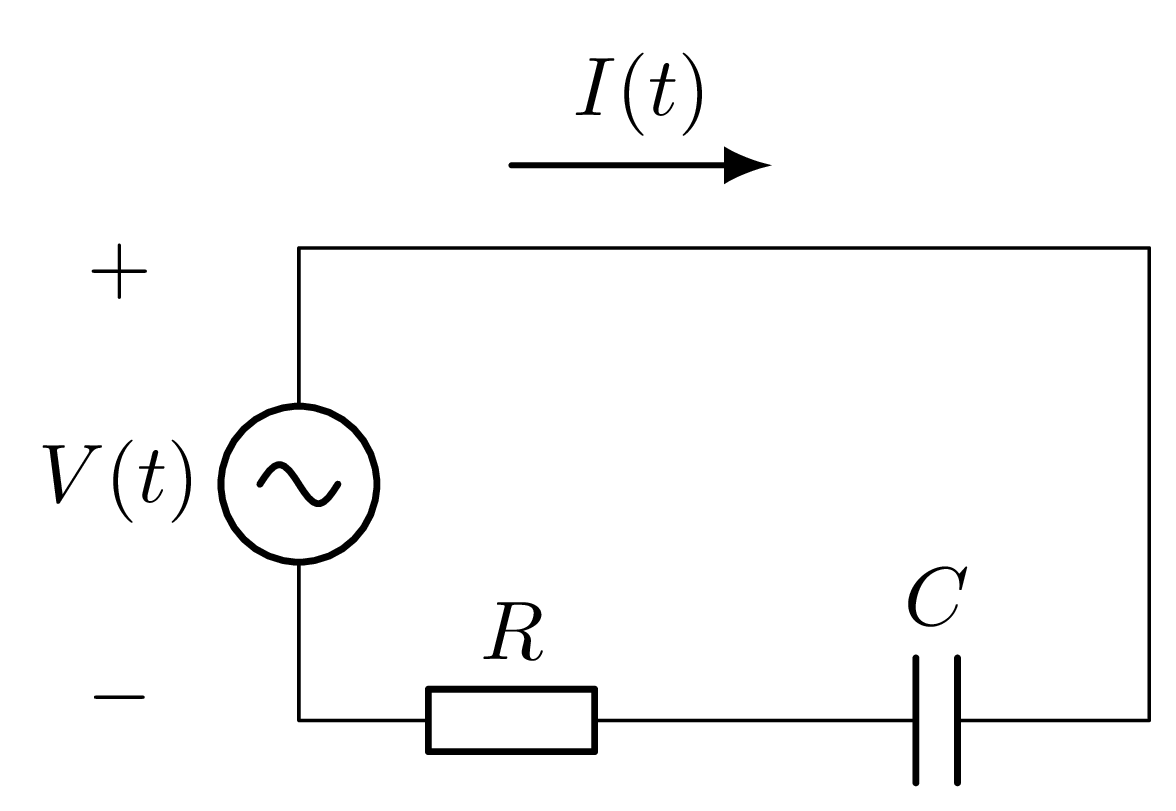
\includegraphics[keepaspectratio,width=40mm]{fig/n32_ex41_zu.png}
\end{zuright}
\begin{komon}
\ko{1} 流れている電流を$I(t)=I_0\sin(\omega t+\varphi)\U{A}$の形に仮定する．このとき，抵抗およびコンデンサーにかかる電圧の瞬時値$V_R(t)$，$V_C(t)$を求めよ．
\ko{2} 抵抗にかかる電圧ベクトル$\overrightarrow{V_R}$およびコンデンサーにかかる電圧ベクトル$\overrightarrow{V_C}$を図示せよ．
\ko{3} 電源電圧ベクトルを図示し，$V_0$および$\omega t$をそれぞれ図に記入せよ．
\ko{4} 以上を用いて，流れる交流電流の最大値$I_0\U{A}$を求めよ．
\ko{5} 電圧と電流の位相のずれの正接$\tan\varphi$を求めよ．
\end{komon}
\end{reidai}

\begin{sisinE}
例題40と同じ手順である．コンデンサーの電圧は電流より$90^\circ$遅れた向きに描く．
\end{sisinE}

\Key{直列接続\ $\Rightarrow$\ 流れる電流$I(t)$が共通．電流ベクトルをもとにして電圧ベクトルを作図}

\begin{kaitou}
\begin{komon}
\ko{1} \[V_R(t)=RI_0\sin(\omega t+\varphi),\quad V_C(t)=\frac{I_0}{\omega C}\sin\Bigl(\omega t+\varphi-\frac{\pi}{2}\Bigr)\Ans\]
\item[{\makebox[1.9zw][r]{(2)(3)}}] 次図のようになる．電源電圧ベクトルは電流ベクトルより$\varphi$だけ遅れている（電流の方が進んでいる）．\Ans
       \begin{center}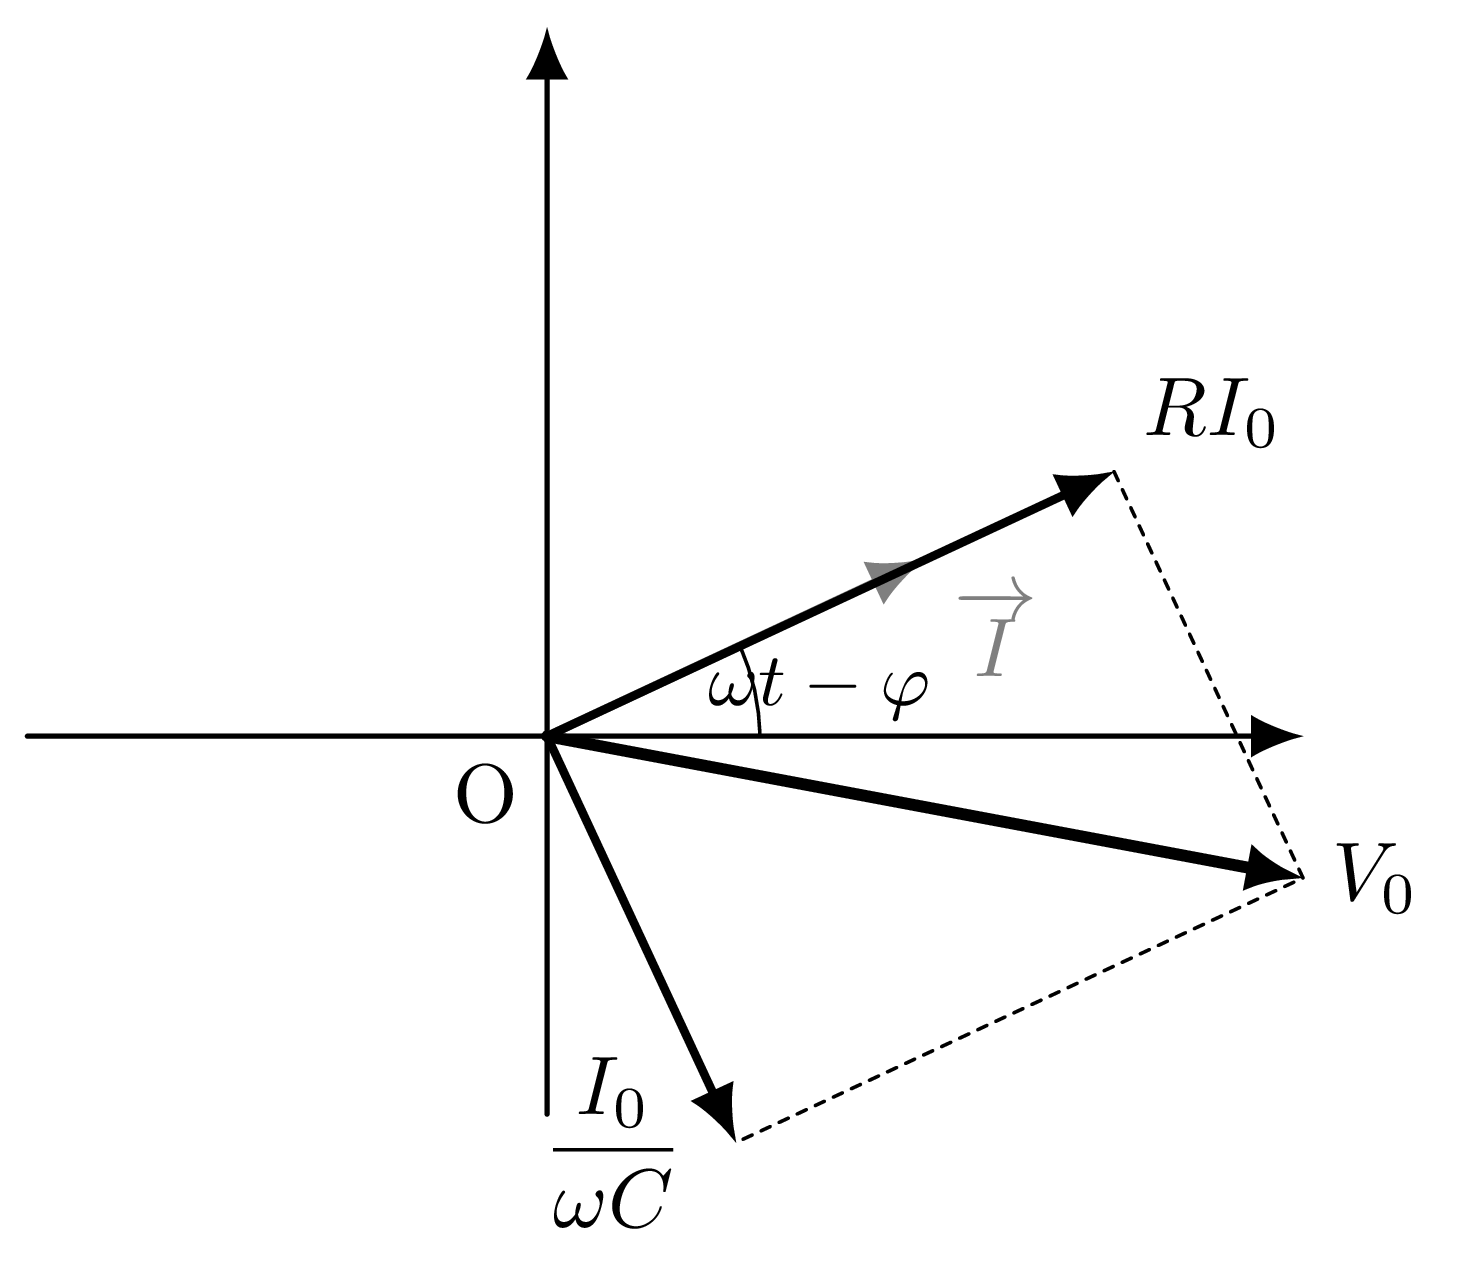
\includegraphics[keepaspectratio,width=52mm]{fig/n32_ex41_ans.png}\end{center}
       （図では電流ベクトルを$x$軸から角$\omega t+\varphi$の向きに描いている．）
\ko{4} \Ana{I_0=\frac{V_0}{\sqrt{R^2+\bigl(\frac{1}{\omega C}\bigr)^2}}\U{A}\Ans}
\ko{5} \[\tan\varphi=\frac{I_0/\omega C}{RI_0}=\frac{1}{\omega CR}\Ans\]
\end{komon}
\end{kaitou}
\end{reidaiunit}

\subsection{RLC直列回路と共振}

電源電圧の最大値$V_0$と流れる電流の最大値$I_0$の比$Z=\dfrac{V_0}{I_0}$を，回路の{\gtfamily インピーダンス}という．
インピーダンスは交流に対する回路全体の電流の流れにくさであり，単位は抵抗と同じ$\U{\Omega}$である（実効値の比でも同じ）．
例題42 で見るように，RLC 直列回路のインピーダンスは
\AnaBD{Z=\sqrt{R^2+\Bigl(\omega L-\frac{1}{\omega C}\Bigr)^2}\U{\Omega}}
となる．この結果は覚えておくとよい．2つの素子だけの直列回路では，無い素子の項を消せばよい．
ただし，インピーダンスからは電流の大きさは分かるが位相差は分からない．位相を問われたらベクトル図を描くこと．

RLC 直列回路で電源の周波数を変えていくと，$\omega L=\dfrac{1}{\omega C}$，すなわち
\AnaBD{f_0=\frac{1}{2\pi\sqrt{LC}}}
のときにインピーダンスが最小（$Z=R$）となり，電流が最大になる．これを{\gtfamily 直列共振}といい，$f_0$を{\gtfamily 共振周波数}という（電気振動の固有周波数と同じ値）．
% 加筆：共振時の特徴（練習［124］）．
共振のときは，コイルとコンデンサーの電圧が大きさが等しく逆向きで打ち消し合い，{\gtfamily 電源電圧がすべて抵抗にかかる}．電流と電源電圧は同位相になり，回路の消費電力は最大になる．
コイルやコンデンサーの電圧そのものは電源電圧より大きくなりうることにも注意（練習［124］）．

%%%%%%%%%%  例題42（原本の【例題45】）  %%%%%%%%%%%%%%%%%%%%
\bsNeed{80mm}
\begin{reidaiunit}
\begin{reidai}{RLC直列回路}
\begin{zuright}{54mm}
\hspace{1zw}抵抗値$R\U{\Omega}$の抵抗，自己インダクタンス$L\U{H}$のコイル，電気容量$C\U{F}$のコンデンサーを，図のように角周波数$\omega\U{rad/s}$の交流電源に接続した．図の$-$側に対する$+$側の電圧の瞬時値が$V(t)=V_0\sin\omega t\U{V}$であるとき，以下の設問に答えよ．
\zusep
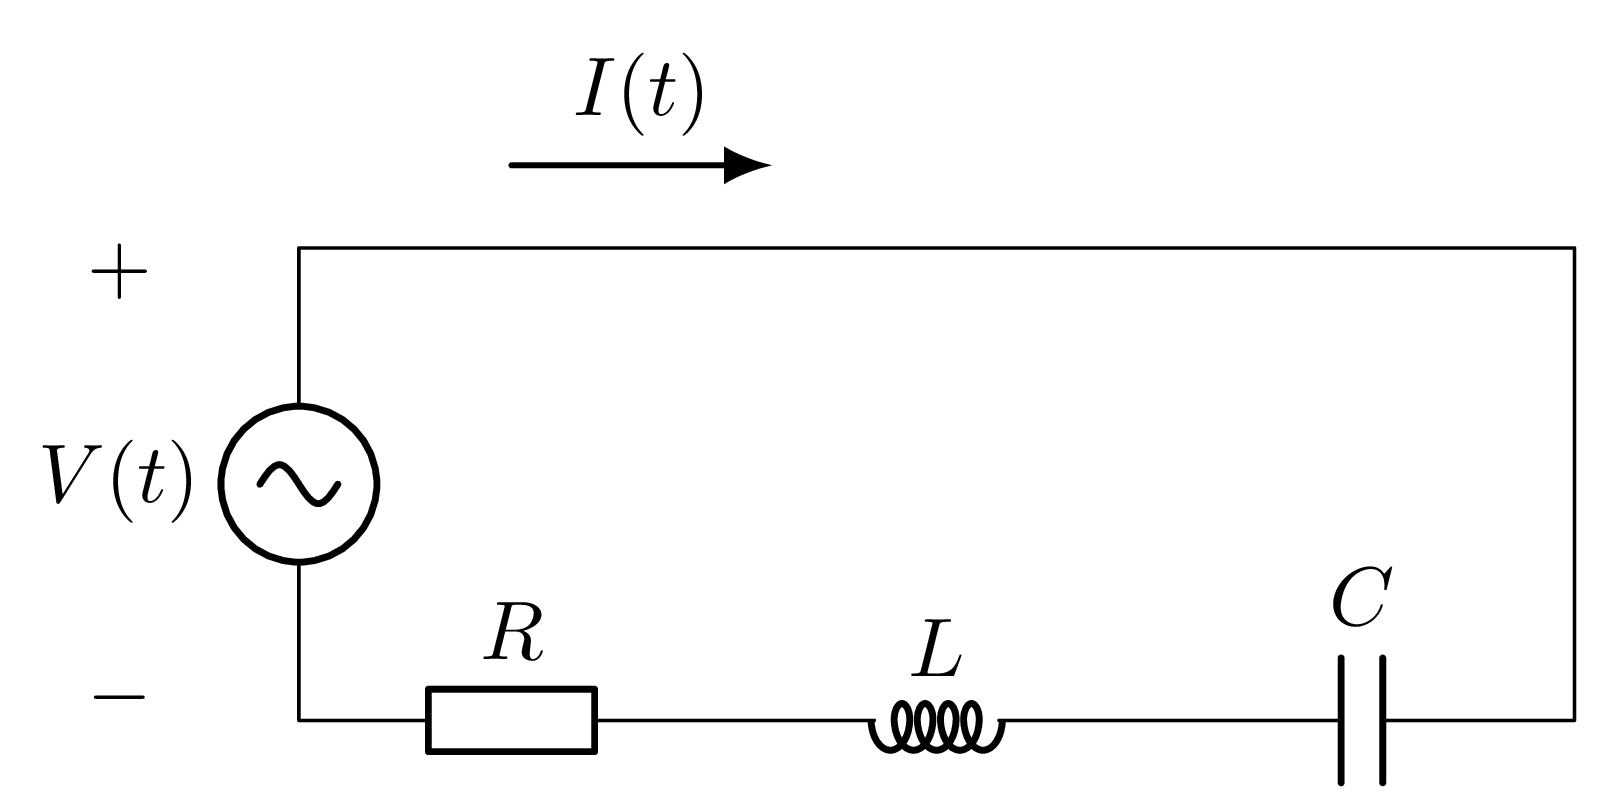
\includegraphics[keepaspectratio,width=52mm]{fig/n32_ex42_zu.png}
\end{zuright}
\begin{komon}
\ko{1} 流れている電流を$I(t)=I_0\sin(\omega t-\varphi)\U{A}$の形に仮定し，これをベクトルで表す．このとき，抵抗・コイル・コンデンサーにかかる電圧ベクトル$\overrightarrow{V_R}$，$\overrightarrow{V_L}$，$\overrightarrow{V_C}$を図示せよ．ただし$\omega L>\dfrac{1}{\omega C}$として作図せよ．
\ko{2} 電源電圧ベクトルを図示し，$V_0$および$\omega t$をそれぞれ図に記入せよ．
\ko{3} 以上を用いて，流れる交流電流の最大値$I_0\U{A}$を求めよ．
\ko{4} 電圧と電流の位相のずれの正接$\tan\varphi$を求めよ．
\ko{5} この回路のインピーダンス$Z=\dfrac{V_0}{I_0}$を求めよ．
\ko{6} 電源の周波数$f\U{Hz}$を変化させていくと，ある周波数で流れる電流の最大値$I_0$が最も大きくなる．このときの電源の周波数$f_0\U{Hz}$（共振周波数）を求めよ．
\end{komon}
\end{reidai}

\begin{sisinE}
コイルの電圧（$90^\circ$進み）とコンデンサーの電圧（$90^\circ$遅れ）は逆向きなので，まずこの2つを合成すると長さ$\bigl(\omega L-\frac{1}{\omega C}\bigr)I_0$のベクトルになる．
これと抵抗の電圧は直交するので三平方の定理が使える．
\end{sisinE}

\Key{直列接続\ $\Rightarrow$\ 電流が共通\quad コイルとコンデンサーの電圧ベクトルは逆向き}

\begin{kaitou}
\begin{komon}
\item[{\makebox[1.9zw][r]{(1)(2)}}] 次図のようになる．\Ans
       \begin{center}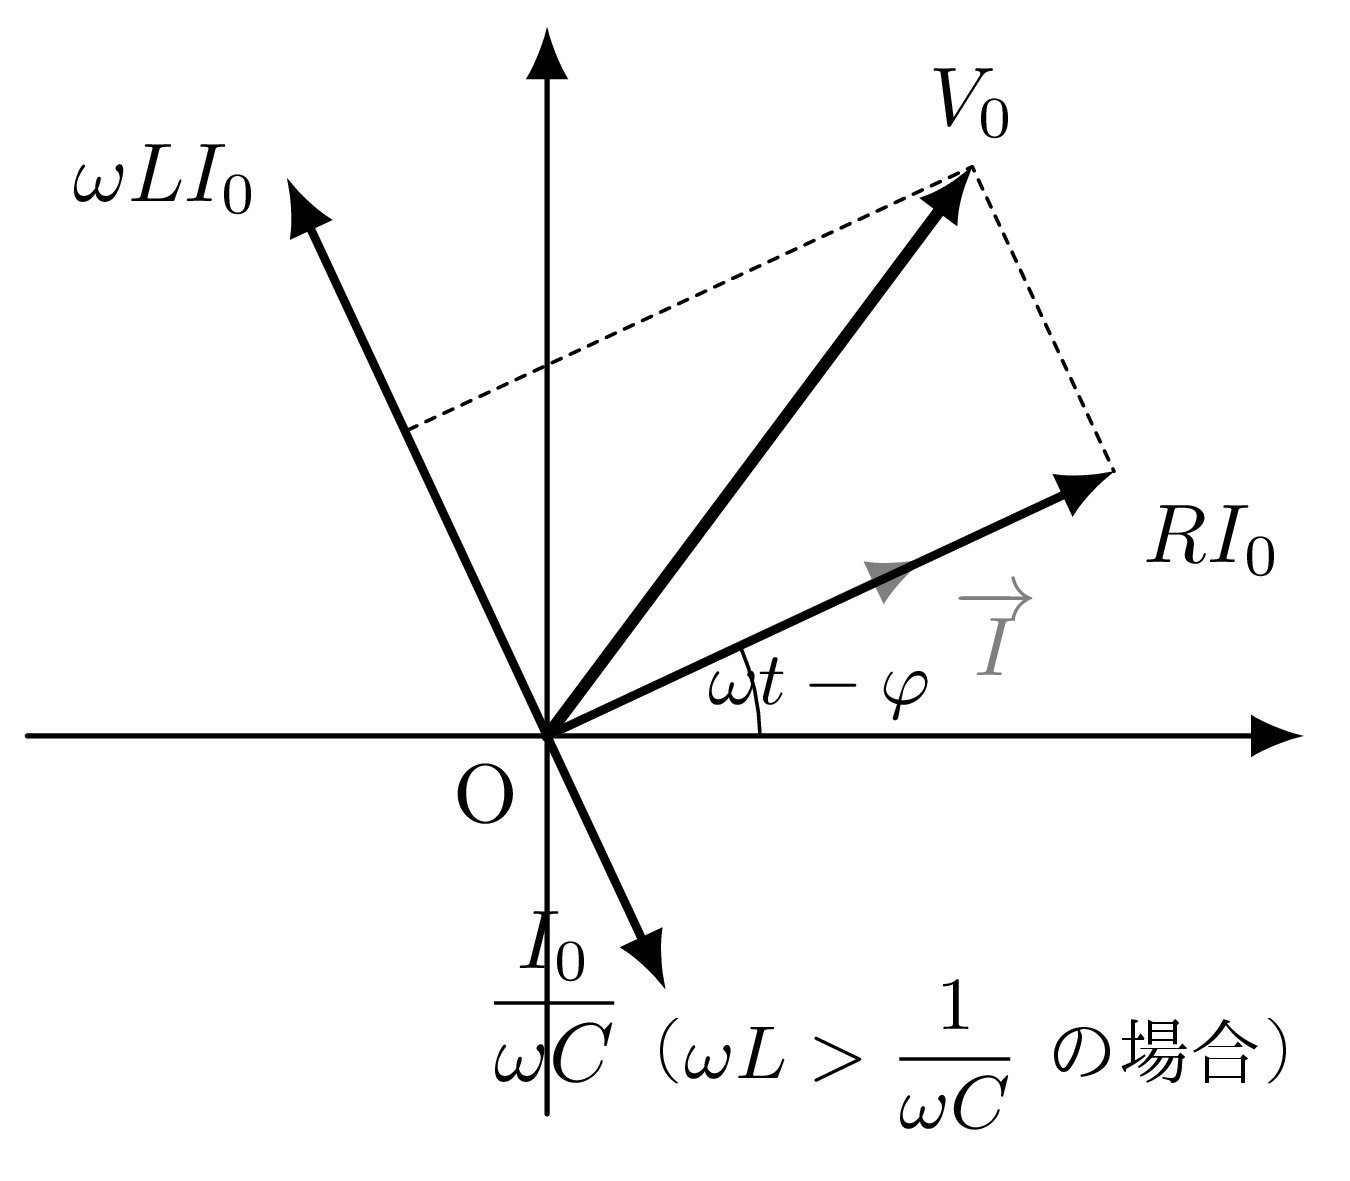
\includegraphics[keepaspectratio,width=52mm]{fig/n32_ex42_ans.png}\end{center}
\ko{3} $V_0^2=(RI_0)^2+\Bigl(\omega LI_0-\dfrac{I_0}{\omega C}\Bigr)^2$より
       \Ana{I_0=\frac{V_0}{\sqrt{R^2+\bigl(\omega L-\frac{1}{\omega C}\bigr)^2}}\U{A}\Ans}
\ko{4} \[\tan\varphi=\frac{\omega L-\frac{1}{\omega C}}{R}\Ans\]
\ko{5} \[Z=\frac{V_0}{I_0}=\sqrt{R^2+\Bigl(\omega L-\frac{1}{\omega C}\Bigr)^2}\U{\Omega}\Ans\]
\ko{6} $I_0$が最大になるのは$Z$が最小，すなわち$\omega L=\dfrac{1}{\omega C}$のときなので$\omega=\dfrac{1}{\sqrt{LC}}$．よって
       \[f_0=\frac{1}{2\pi\sqrt{LC}}\U{Hz}\Ans\]
\end{komon}
\end{kaitou}
\end{reidaiunit}

\bsNeed{30mm}
\begin{matome}{インピーダンスと直列共振}
 \hspace{3mm} RLC 直列回路のインピーダンス\quad $Z=\dfrac{V_0}{I_0}=\sqrt{R^2+\Bigl(\omega L-\dfrac{1}{\omega C}\Bigr)^2}$\\
 \hspace{3mm} 共振周波数\quad $f_0=\dfrac{1}{2\pi\sqrt{LC}}$\quad（$Z=R$で最小，電流最大，電源電圧がすべて抵抗にかかる）
\end{matome}

\bsNeed{70mm}
\subsection{複雑な交流回路}

並列部分を含む回路でも，電流ベクトル図と電圧ベクトル図を組み合わせれば解くことができる．

\bsNeed{44mm}
\begin{matome}{複雑な交流回路の解き方}
 \MARU{1}\ 回路の中で共通になっているものを探す（直列部分なら\AnaB{電流}，並列部分なら\AnaB{電圧}が共通）\\
 \MARU{2}\ \MARU{1}の共通の量の大きさ・位相を仮定してベクトルで描く\\
 \MARU{3}\ それをもとに，各素子の電圧・電流のベクトルを描いていく\\
 \MARU{4}\ 電源電圧がどのベクトルの和になっているかを考え，三平方の定理などを使う
\end{matome}
問題文の誘導の順番に考える前に，先にベクトル図を描いてしまってから考える方が簡単なことも多い．

% 加筆：並列共振と周波数によるふるまい（練習［126］）．
コイルとコンデンサーを{\gtfamily 並列}につなぐと，両者には同じ電圧がかかり，コイルの電流（電圧より$90^\circ$遅れ）とコンデンサーの電流（$90^\circ$進み）は逆向きになる．
$\omega C=\dfrac{1}{\omega L}$のときは2つの電流の大きさが等しく打ち消し合うので，並列部分全体には電流が流れ込まない（LC の間を電流が行き来するだけ）．これを{\gtfamily 並列共振}という．共振周波数は直列共振と同じ$\dfrac{1}{2\pi\sqrt{LC}}$だが，並列共振では電源からの電流が最小（$0$）になる．
また，$X_L=\omega L$，$X_C=\dfrac{1}{\omega C}$より，{\gtfamily 周波数が非常に高いとコイルは断線，コンデンサーはただの導線}のように，{\gtfamily 周波数が非常に低い（直流に近い）とコイルはただの導線，コンデンサーは断線}のようにふるまう．

%%%%%%%%%%  例題43（原本の【例題46】）  %%%%%%%%%%%%%%%%%%%%
\bsNeed{70mm}
\begin{reidaiunit}
\begin{reidai}{複雑な交流回路}
\begin{zuright}{56mm}
\hspace{1zw}抵抗値$R\U{\Omega}$の抵抗，自己インダクタンス$L\U{H}$のコイル，電気容量$C\U{F}$のコンデンサーを用いて図のような回路を作る．今，この回路の$\mathrm{AD}$間に周波数$60\U{Hz}$の交流電源を加えたところ，$\mathrm{C}$点に対する$\mathrm{B}$点の電位$V_{\mathrm{BC}}\U{V}$は下のグラフのように時間変化をした．この周波数に対しては，$R=120\U{k\Omega}$，$\omega L=60\U{k\Omega}$，$\dfrac{1}{\omega C}=120\U{k\Omega}$であるものとして，以下の問いに答えよ．
\zusep
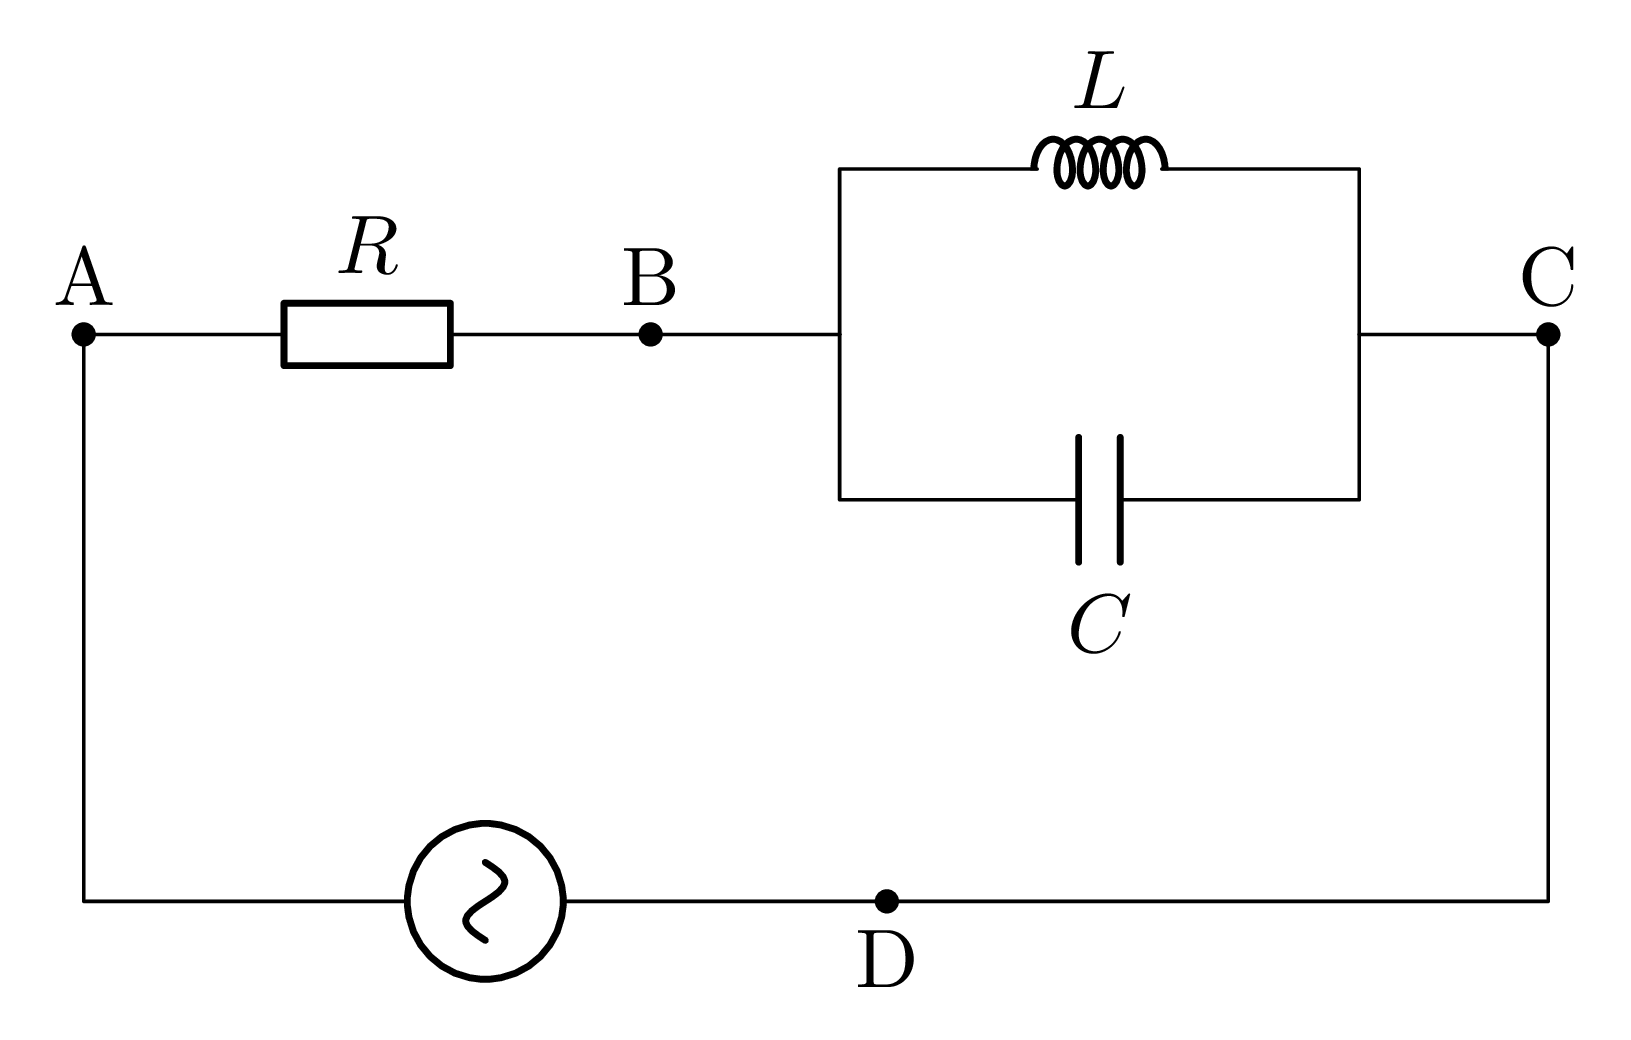
\includegraphics[keepaspectratio,width=54mm]{fig/n32_ex43_zu.png}\\[2mm]
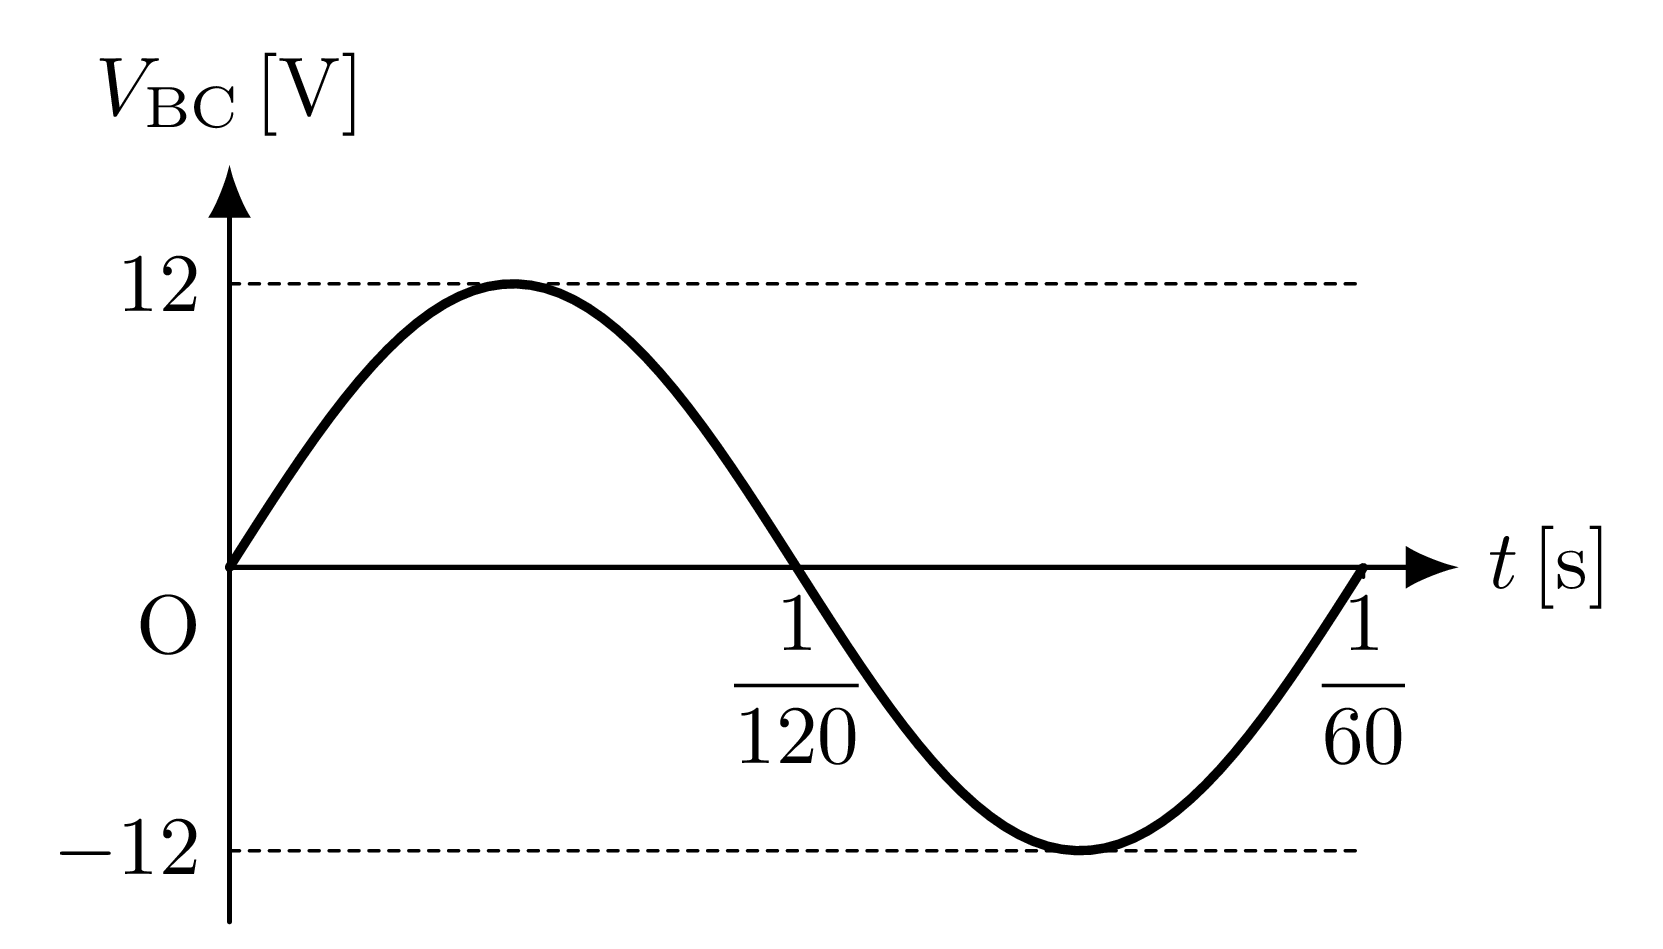
\includegraphics[keepaspectratio,width=48mm]{fig/n32_ex43_graph.png}
\end{zuright}
\begin{komon}
\ko{1} コイルを流れる電流$I_L(t)\U{A}$，コンデンサーを流れる電流$I_C(t)\U{A}$が時刻$t$に対してどのように変化するのか，その式を示せ．ただし，電流が$\mathrm{B}$から$\mathrm{C}$の向きに流れる場合を正とする．
\ko{2} $\mathrm{B}$に対する$\mathrm{A}$の電位$V_{\mathrm{AB}}(t)\U{V}$，および$\mathrm{D}$に対する$\mathrm{A}$の電位$V_{\mathrm{AD}}(t)\U{V}$の時間変化を式で表せ．
\end{komon}
\end{reidai}

\begin{sisinE}
コイルとコンデンサーは並列なので，共通の電圧$V_{\mathrm{BC}}(t)=12\sin\omega t$（$\omega=120\pi$）を基準にする．
それぞれの電流を最大値と位相から求め，その和が抵抗を流れる電流である．
\end{sisinE}

\Key{交流回路\ $\Rightarrow$\ 電流ベクトルと電圧ベクトルを併用して考える}

\begin{kaitou}
\begin{komon}
\ko{1} グラフより$V_{\mathrm{BC}}(t)=12\sin\omega t\U{V}$（$\omega=2\pi\times 60=120\pi\U{rad/s}$）．コイルの電流は最大値$\dfrac{12}{60\times 10^3}=2.0\times 10^{-4}\U{A}$で位相が$\dfrac{\pi}{2}$遅れ，コンデンサーの電流は最大値$\dfrac{12}{120\times 10^3}=1.0\times 10^{-4}\U{A}$で位相が$\dfrac{\pi}{2}$進むので
       \Ana{I_L(t)=-2.0\times 10^{-4}\cos 120\pi t\U{A},\qquad I_C(t)=1.0\times 10^{-4}\cos 120\pi t\U{A}\Ans}
\ko{2} 抵抗には$\mathrm{A}\to\mathrm{B}$の向きに$I_L+I_C=-1.0\times 10^{-4}\cos 120\pi t$が流れるので
       \[V_{\mathrm{AB}}(t)=R(I_L+I_C)=-12\cos 120\pi t\U{V}\Ans\]
       $\mathrm{C}$と$\mathrm{D}$は導線でつながっているので
       \[\begin{aligned}
         V_{\mathrm{AD}}(t)&=V_{\mathrm{AB}}+V_{\mathrm{BC}}=12\sin 120\pi t-12\cos 120\pi t\\
         &=12\sqrt{2}\sin\Bigl(120\pi t-\frac{\pi}{4}\Bigr)\U{V}
       \end{aligned}\Ans\]
       \begin{chuu}
       並列部分では，コイルの電流の方が大きいので，並列部分全体は「コイル」のようにふるまい，電流は電圧$V_{\mathrm{BC}}$より$\dfrac{\pi}{2}$遅れている．
       \end{chuu}
\end{komon}
\end{kaitou}
\end{reidaiunit}

\subsection{電磁波}

\begin{center}

\includegraphics[keepaspectratio,width=100mm]{text2_p93_fig1.png}
\end{center}

磁場が時間変化すると，電磁誘導によってその周りに電場（誘導電場，30.2）が生じる．
これと対になる現象として，{\gtfamily 電場が時間変化すると，その周りに磁場が生じる}ことが知られている．
そのため，ある点の電場が変化するとその周りに磁場が生じ，その磁場の変化がさらに新たな電場を生む，ということが繰り返され，電場と磁場の振動が空間を伝わっていく．これを{\gtfamily 電磁波}という．
電磁波には次のような特徴がある．
\begin{description}
\item[\MARU{1}] 電場と磁場の波が同時に伝わっていく．
\item[\MARU{2}] 電磁波は\AnaB{横波}である（進行方向に垂直に振動する）．
\item[\MARU{3}] 電場の振動方向と磁場の振動方向は互いに垂直である．
\end{description}
電磁波の伝わる速さ$c$は，空間の誘電率$\varepsilon$と透磁率$\mu$を用いて
\[c=\frac{1}{\sqrt{\varepsilon\mu}}\]
と書ける．真空中では$c=\dfrac{1}{\sqrt{\varepsilon_0\mu_0}}\fallingdotseq 3.00\times 10^8\U{m/s}$であり，光の速さに等しい．光も電磁波の一種である．

\begin{zuright}{62mm}
\hspace{1zw}電磁波も波であるから，波長$\lambda$と振動数$f$の間に$c=f\lambda$の関係が成り立つ．電磁波は波長（振動数）によって右図のように分類される．
{\gtfamily 電波・赤外線・可視光・紫外線・X線・$\gamma$線はすべて電磁波}であり，波長が異なるだけである．

\hspace{1zw}可視光は波長がおよそ$380\sim 780\U{nm}$の電磁波で，長波長側から赤，橙，黄，緑，青，藍，紫の順に並ぶ．赤より長い側が赤外線，紫より短い側が紫外線である．波長が短いほど（振動数が大きいほど）光子1個のエネルギーが大きい（第5章）．

\hspace{1zw}電磁波は，LC 回路の電気振動（31.2）で生じる振動電流をアンテナに流すことで発生させることができる（練習［129］）．電荷が振動すると周りの電場が振動し，それが磁場を生み……と電磁波が放射される．
\zusep

\includegraphics[keepaspectratio,width=60mm]{text2_p93_fig2.png}
\end{zuright}

% 加筆：リサジュー図形（練習［131］の前提）．
\noindent{\gtfamily 参考：オシロスコープとリサジュー図形}\quad
ブラウン管（第29回の例題26 の電場偏向を利用した装置）の$x$方向，$y$方向の偏向板に交流電圧をかけると，輝点は各瞬間の電圧に比例した位置に来る．
周波数が高いと輝点の動きは目で追えず，軌跡全体が光って見える．$x$方向だけに$V_0\sin\omega t$をかければ$x$軸上の線分，$x$，$y$の両方に同位相の電圧をかければ斜めの線分，位相が$\dfrac{\pi}{2}$ずれていれば楕円（振幅が等しければ円）が見える．このような図形を{\gtfamily リサジュー図形}といい，2つの電圧の位相差を目で見ることができる（練習［131］）．

\bsNeed{30mm}
\begin{matome}{電磁波}
 \hspace{3mm} 電場と磁場の振動が伝わる\AnaB{横波}．電場と磁場の振動方向は互いに垂直．真空中の速さ$c=\dfrac{1}{\sqrt{\varepsilon_0\mu_0}}\fallingdotseq 3.00\times 10^8\U{m/s}$\\
 \hspace{3mm} 波長の長い順に\quad 電波 → 赤外線 → 可視光（赤〜紫） → 紫外線 → X線 → $\gamma$線
\end{matome}

\newpage

%%%%%%%%%%%%%%%%%%%%  練習問題  %%%%%%%%%%%%%%%%%%%%
% 第31回の［119］に続く．
\setcounter{qno}{119}

\filbreak
\Rank{A問題}

\Mon{基本公式の確認}

\hspace{1zw}以下の設問に答えよ．ただし，$\sqrt{2}\fallingdotseq 1.41$，$\pi\fallingdotseq 3.14$として具体値で答えよ．
\begin{komon}
\ko{1} 周波数$50\U{Hz}$の交流電源に対して抵抗値$5\U{\Omega}$の抵抗，自己インダクタンス$\dfrac{1.12}{\pi}\U{H}$のコイル，そして電気容量$\dfrac{100}{\pi}\U{\mu F}$のコンデンサーを直列につないだとき，この回路のインピーダンスは何$\U{\Omega}$か．
\ko{2} 周波数$50\U{Hz}$の交流電源に対して抵抗値$24\U{\Omega}$の抵抗，電気容量$\dfrac{10^4}{7\pi}\U{\mu F}$のコンデンサーを直列につないだとき，この回路のインピーダンスは何$\U{\Omega}$か．
\ko{3} 周波数$50\U{Hz}$の交流電源に対して抵抗値$10\U{\Omega}$の抵抗，自己インダクタンス$\dfrac{100}{\pi}\U{mH}$のコイルを直列につないだとき，この回路のインピーダンスは何$\U{\Omega}$か．ただしコイルの抵抗は無視できるものとする．
\end{komon}

\Mon{電磁波の分類}

\hspace{1zw}次の(1)から(6)の中から電磁波を選び出し，波長の長いものから順に並べよ．\\
\hspace*{2zw}(1)\ 可視光線\hspace{8mm}(2)\ 紫外線\hspace{8mm}(3)\ X線\hspace{8mm}(4)\ 赤外線\hspace{8mm}(5)\ ラジオ放送の波\hspace{8mm}(6)\ テレビ放送の波

\filbreak
\Rank{B問題}

\Mon{RL直列回路}

\begin{zuright}{34mm}
\hspace{1zw}右図のように抵抗値$100\U{\Omega}$の抵抗体$\mathrm{R}$と自己インダクタンス$0.159\U{H}$のコイル$\mathrm{L}$を，電圧$100\U{V}$，周波数$100\U{Hz}$の交流電源に直列に接続した．この回路について，以下の設問に答えよ．
\begin{komon}
\ko{1} この回路に流れる電流の実効値を求めよ．
\ko{2} 流れる電流と電源電圧の位相差はいくらか．ただし，電源電圧に対して流れる電流の位相が進んでいる場合をプラスとして答えよ．
\ko{3} 抵抗およびコイルの各素子にかかる電圧の実効値を求めよ．
\ko{4} この回路の全インピーダンス$Z$を求めよ．
\end{komon}
\zusep
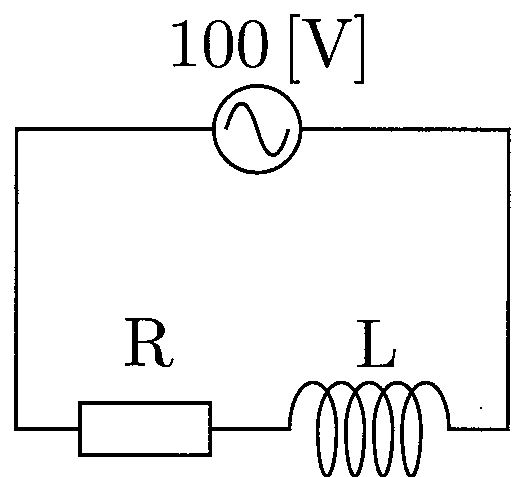
\includegraphics[keepaspectratio,width=30mm]{fig/n32_p122_zu.png}
\end{zuright}

\Mon{RC直列回路}

\begin{zuright}{30mm}
\hspace{1zw}一定周波数$f_0\U{Hz}$，一定交流電圧$10.0\U{V}$の交流電源がある．まず，図1のように，この電源に電気容量$0.10\U{\mu F}$のコンデンサー$\mathrm{C}_1$と，電気容量の未知のコンデンサー$\mathrm{C}_2$を直列につなぎ，コンデンサー$\mathrm{C}_2$の極板間にかかる交流電圧を測定したところ，$8.0\U{V}$であった．
\begin{komon}
\ko{1} コンデンサー$\mathrm{C}_2$の電気容量を求めよ．
\end{komon}
\hspace{1zw}次に，図2のように交流電源とコンデンサー$\mathrm{C}_2$はそのままにして，コンデンサー$\mathrm{C}_1$のかわりに$30\U{k\Omega}$の抵抗$\mathrm{R}$をつなぎ，コンデンサー$\mathrm{C}_2$にかかる交流電圧を測定したところ，同じく$8.0\U{V}$であった．
\zusep
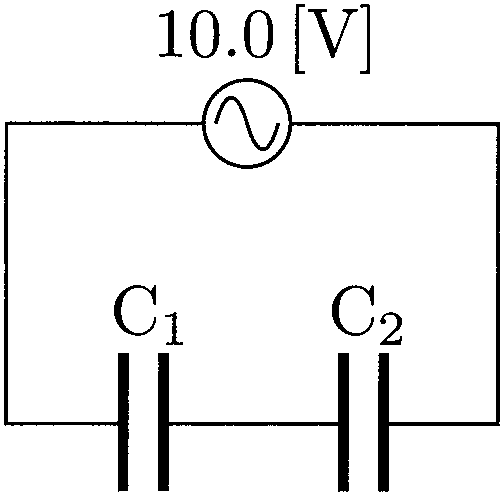
\includegraphics[keepaspectratio,width=28mm]{fig/n32_p123_zu1.png}\\[1mm]{\small 図1}\\[2mm]
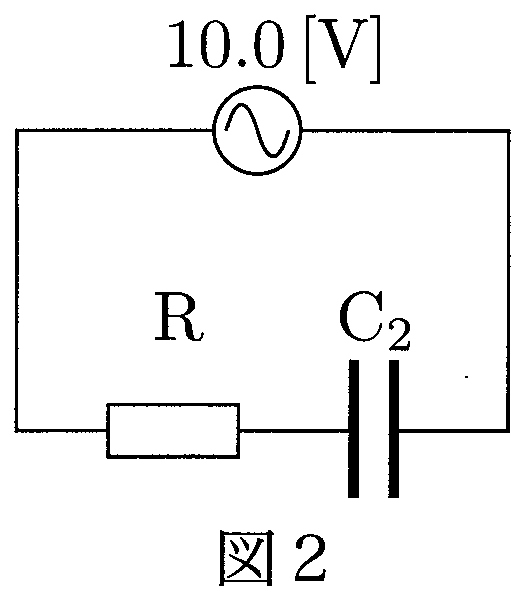
\includegraphics[keepaspectratio,width=28mm]{fig/n32_p123_zu2.png}
\end{zuright}
\begin{komon}
\ko{2} 抵抗$\mathrm{R}$にかかる交流電圧を求めよ．
\ko{3} 回路に流れている交流電流を求めよ．
\ko{4} 回路のインピーダンス$Z$を求めよ．
\ko{5} 交流電源の周波数$f_0$を求めよ．
\end{komon}

\Mon[\Sitei]{RLC直列共振回路}

\hspace{1zw}可変抵抗$\mathrm{R}$，自己インダクタンス$0.40\U{H}$のコイル$\mathrm{L}$，電気容量$1.0\times 10^{-5}\U{F}$のコンデンサー$\mathrm{C}$を直列接続し，その両端に周波数を変えることのできる，実効電圧$10\U{V}$の交流電源を接続した．電源の周波数を少しずつ変えていったところ，ある周波数のときに直列共振が起きたという．これについて，以下の設問に答えよ．
\begin{komon}
\ko{1} 共振周波数を求めよ．
\ko{2} 直列共振の状態はどのような特徴があるか．簡単に述べよ．
\ko{3} このときコイル$\mathrm{L}$にかかる電圧が$100\U{V}$になるためには，可変抵抗$\mathrm{R}$の抵抗値をいくらにすればよいか．
\ko{4} (3)のとき，コンデンサーにかかる電圧を求めよ．
\end{komon}

\Mon{電流・電圧グラフの読み取り}

\begin{zuright}{50mm}
\hspace{1zw}図1のように抵抗$\mathrm{R}$とコイル$\mathrm{L}$を直列につなぎ，その両端にある交流電源をつなげたところ，時刻$t\U{s}$における交流電源の$-$に対する$+$の電位$V(t)\U{V}$および図の矢印の向きに回路を流れる電流$I(t)\U{A}$はそれぞれ図2，図3のようになっていたという．これについて，以下の設問に答えよ．
\begin{komon}
\ko{1} この交流電源の周波数および電圧を求めよ．
\ko{2} 抵抗$\mathrm{R}$の抵抗値$R\U{\Omega}$を求めよ．
\ko{3} コイル$\mathrm{L}$の自己インダクタンス$L\U{H}$を求めよ．
\end{komon}
\zusep
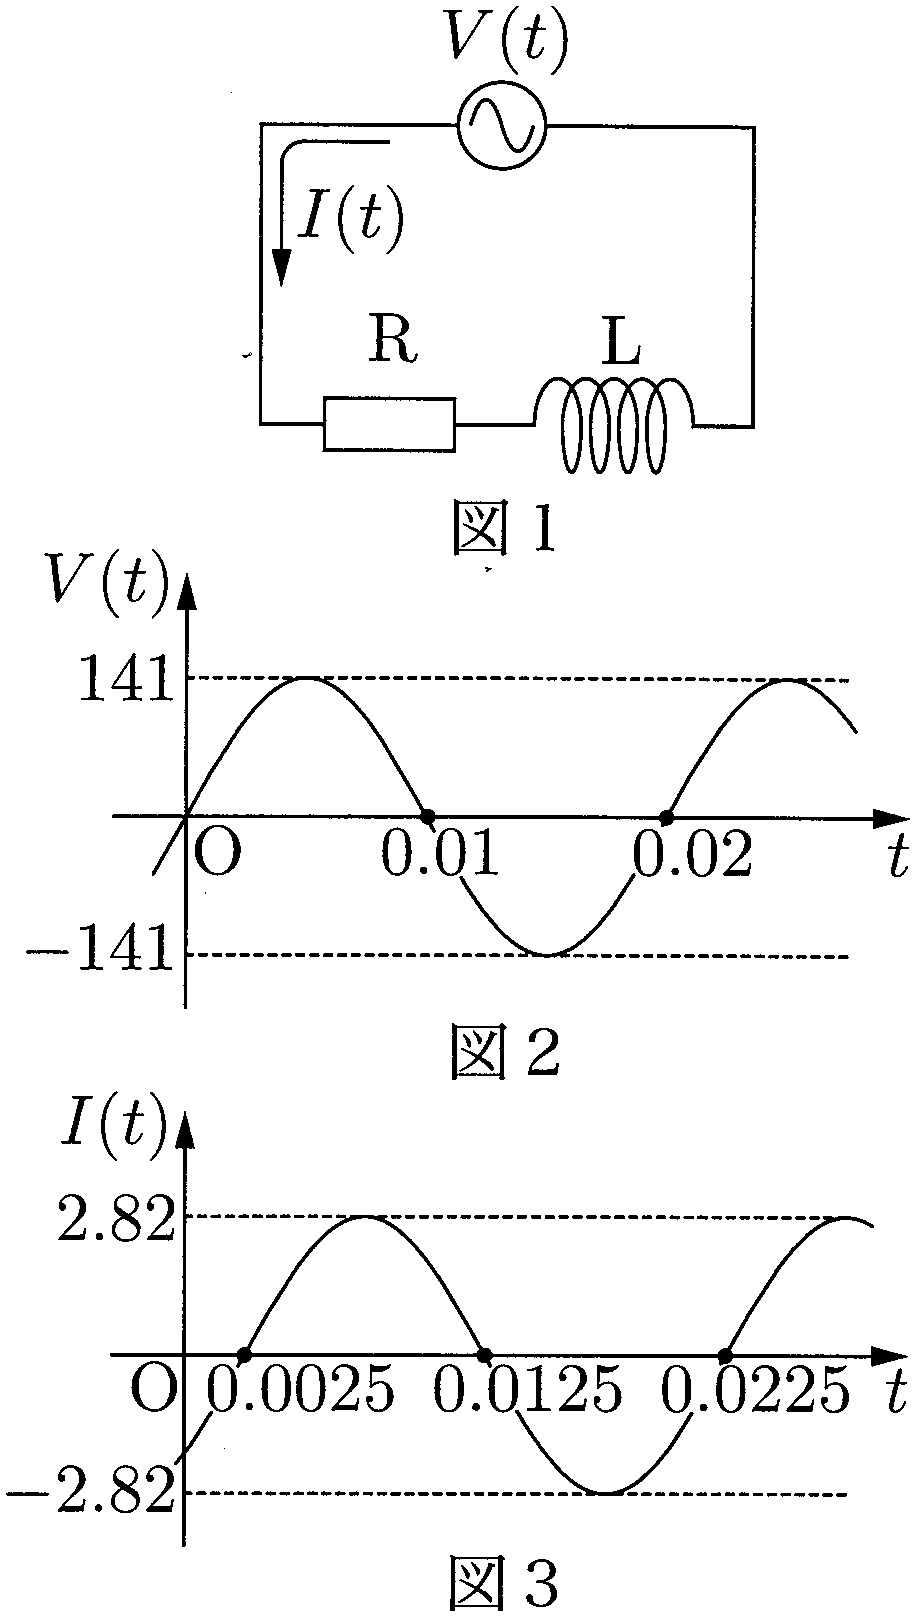
\includegraphics[keepaspectratio,width=48mm]{fig/n32_p125_zu.png}
\end{zuright}

\Mon[\Sitei]{並列共振回路}

\begin{zuright}{40mm}
\hspace{1zw}右図のように抵抗値$R\U{\Omega}$の抵抗$\mathrm{R}$，自己インダクタンス$L\U{H}$のコイル$\mathrm{L}$，そして電気容量$C\U{F}$のコンデンサー$\mathrm{C}$を接続し，右図の$-$に対する$+$の電圧の瞬時値が$V(t)=V_0\sin 2\pi ft\U{V}$で表される交流電源をつなげた．コイルの抵抗は無視できるとして，以下の設問に答えよ．
\begin{komon}
\ko{1} 電源の周波数$f\U{Hz}$を$0\U{Hz}$から次第に増していくと，$f_0\U{Hz}$のとき抵抗$\mathrm{R}$を流れる電流が$0\U{A}$になった．このときの$f_0$の値を求めよ．
\ko{2} 電源の周波数$f$を無限に大きくしたときの，抵抗体$\mathrm{R}$を流れる電流の実効値を求めよ．
\end{komon}
\zusep
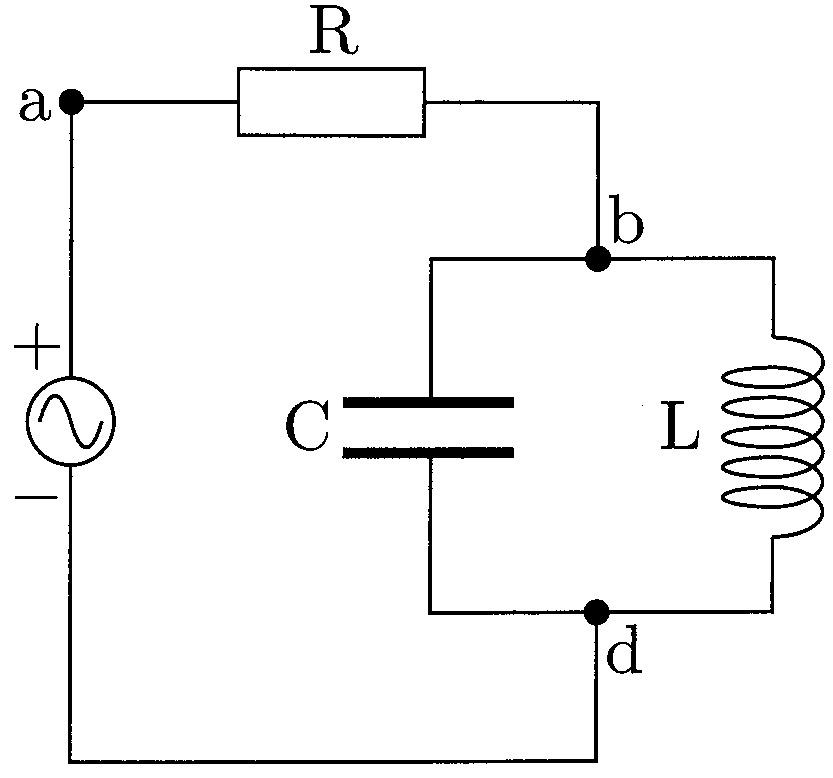
\includegraphics[keepaspectratio,width=38mm]{fig/n32_p126_zu.png}
\end{zuright}

\Mon{複雑な交流回路}

\begin{zuright}{56mm}
\hspace{1zw}抵抗値が$2R$，$3R$，$6R\U{\Omega}$の電気抵抗$\mathrm{R}_1\sim\mathrm{R}_3$，容量リアクタンスが$6R\U{\Omega}$のコンデンサー$\mathrm{C}$，実効電圧が$\overline{V}\U{V}$の交流電源$\mathrm{V}$を用いて右図のような回路を作った．今，抵抗$\mathrm{R}_2$に流れる交流電流の実効値を$\overline{I_2}\U{A}$とおく．これについて以下の設問に答えよ．
\begin{komon}
\ko{1} 抵抗$\mathrm{R}_3$にかかる交流電圧の実効値を$\overline{I_2}$を用いて表せ．
\ko{2} 抵抗$\mathrm{R}_1$を流れる交流電流の実効値を$\overline{I_2}$を用いて表せ．
\ko{3} (1)，(2)などから，抵抗$\mathrm{R}_2$に流れる交流電流の実効値$\overline{I_2}$を求めよ．
\end{komon}
\zusep
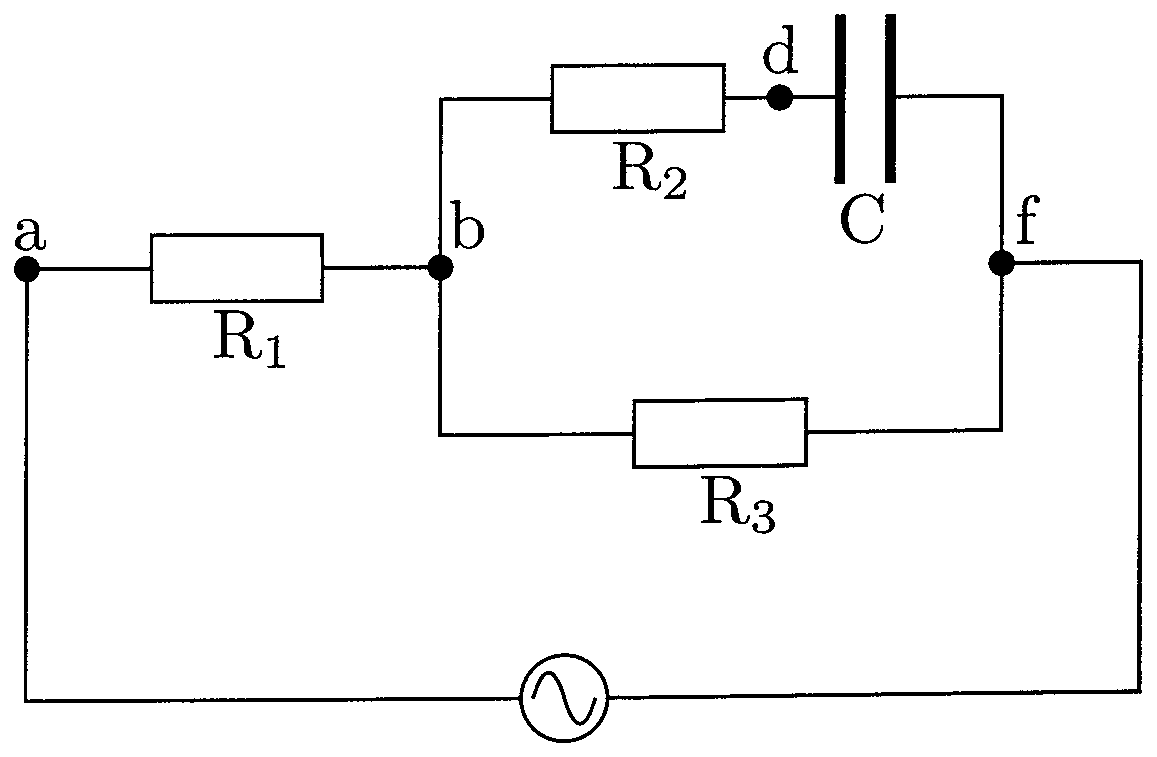
\includegraphics[keepaspectratio,width=54mm]{fig/n32_p127_zu.png}
\end{zuright}

\filbreak
\Rank{C問題}

\Mon{直流・交流回路}

\begin{zuright}{54mm}
\hspace{1zw}図1のように抵抗体$\mathrm{R}$とコイル$\mathrm{L}$とからなる回路に，直流と交流を測定することのできる電流計$\mathrm{A}$と電圧計$\mathrm{V}$とをつないだ．まず端子$\mathrm{P}$，$\mathrm{Q}$に直流電源をつなぎ，電圧を$0\U{V}$からゆるやかに上げていき，電圧計$\mathrm{V}$と電流計$\mathrm{A}$を直流測定にしてその目盛りを読みとったところ，図2の(a)に示すような関係を得た．次に周波数$60\U{Hz}$の交流電源を端子$\mathrm{P}$，$\mathrm{Q}$につなぎ，電圧を$0\U{V}$からゆるやかに上げていき，電圧計$\mathrm{V}$と電流計$\mathrm{A}$を交流測定にしてその目盛りを読みとったところ，図2の(b)で示すような関係を得た．なお，交流測定状態にした場合には電流・電圧の実効値が読み取られる．以下の設問に答えよ．
\begin{komon}
\ko{1} 抵抗$\mathrm{R}$の抵抗値$R\U{\Omega}$を求めよ．
\ko{2} 交流の場合，回路のインピーダンス$Z\U{\Omega}$を求めよ．
\ko{3} コイル$\mathrm{L}$の自己インダクタンス$L\U{H}$を求めよ．
\end{komon}
\zusep
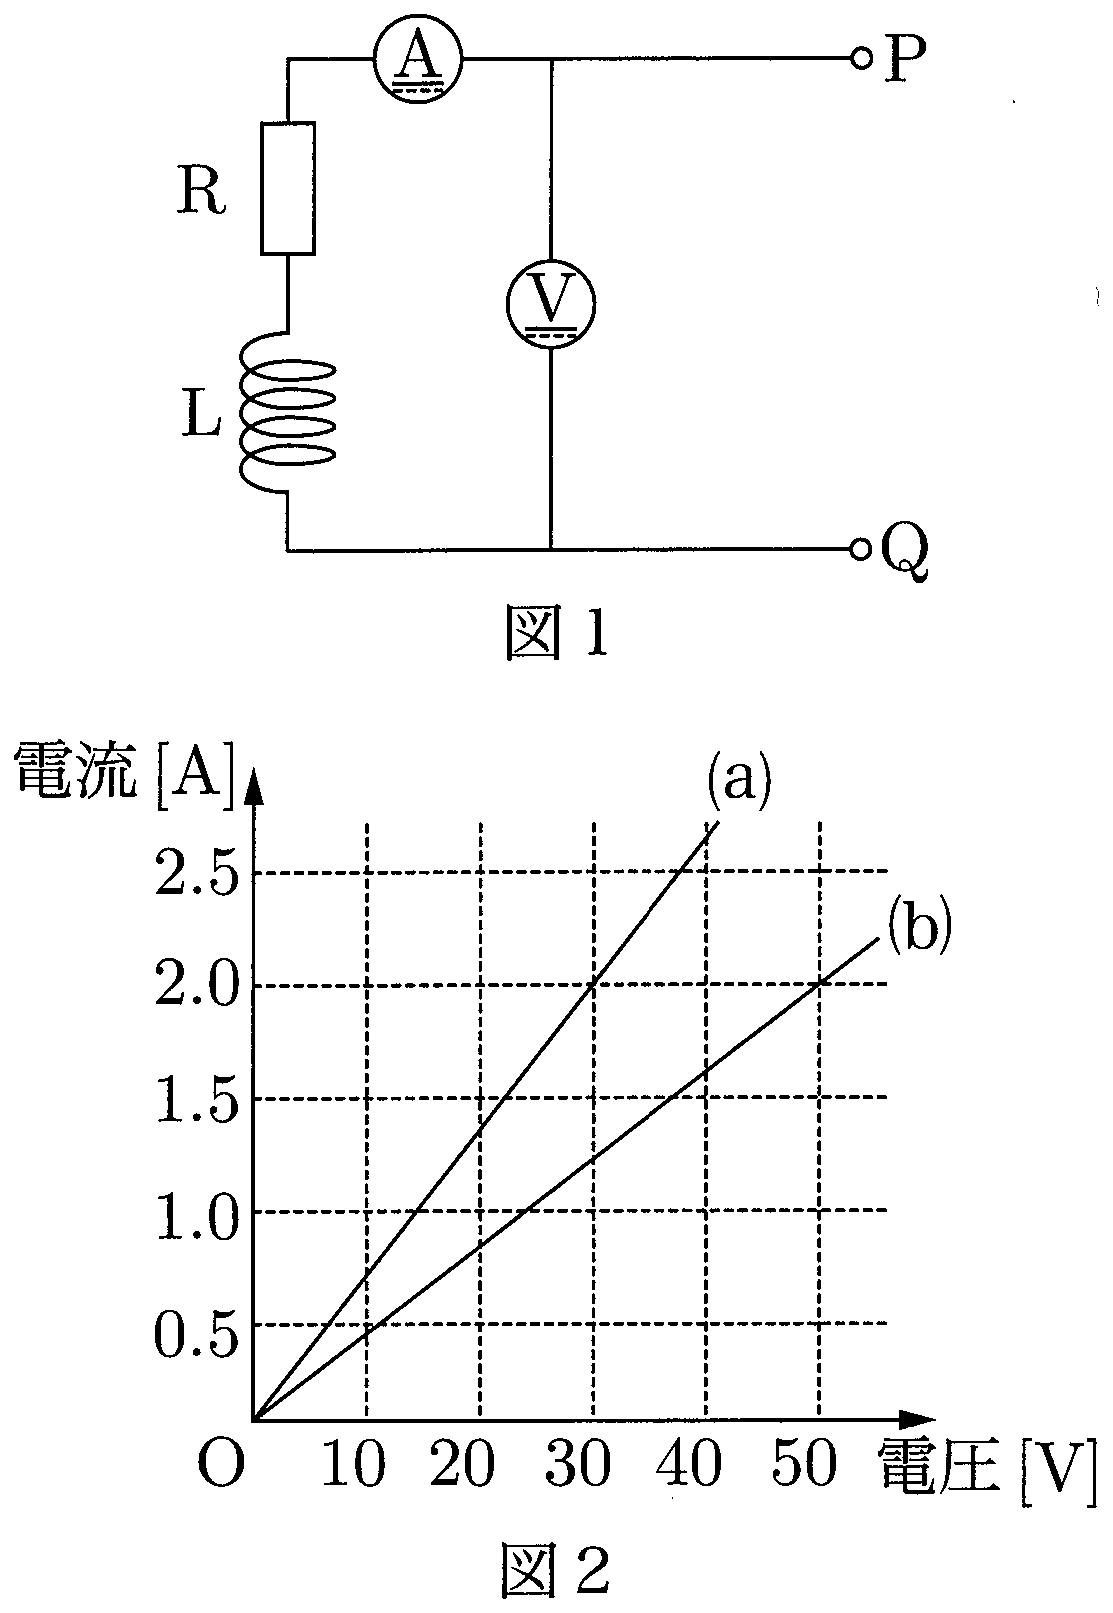
\includegraphics[keepaspectratio,width=52mm]{fig/n32_p128_zu.png}
\end{zuright}

\Mon{電磁波の発生}

\begin{zuright}{50mm}
\hspace{1zw}以下の\framebox[4zw]{\rule{0pt}{1.1zw}1}〜\framebox[4zw]{\rule{0pt}{1.1zw}8}に適当な式または語句を入れよ．
\par
\hspace{1zw}右図のような回路において，コンデンサー$\mathrm{C}$を充電しておく．スイッチ$\mathrm{S}$を閉じると，電荷はコイル$\mathrm{L}$を通って放電されるが，コイル$\mathrm{L}$との\framebox[4zw]{\rule{0pt}{1.1zw}1}のために電荷は打ち消し合って止まってしまうことなくコンデンサー$\mathrm{C}$の両極板間を往復する．
\zusep
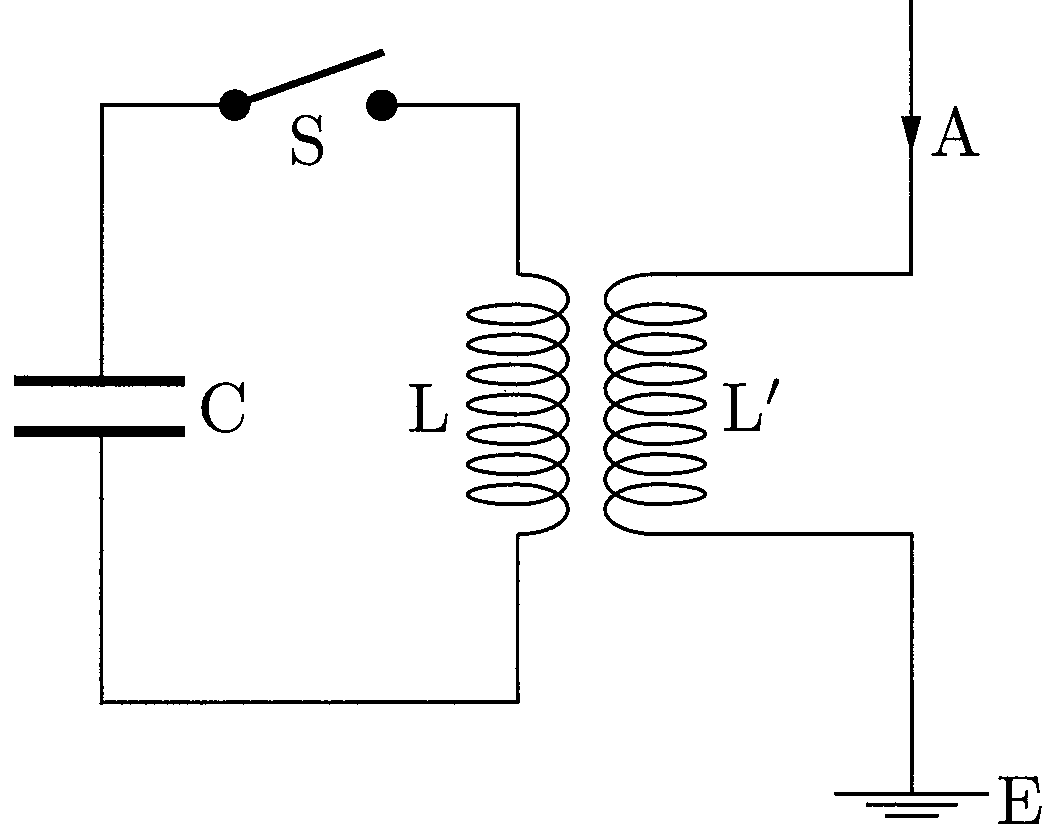
\includegraphics[keepaspectratio,width=48mm]{fig/n32_p129_zu.png}
\end{zuright}
コンデンサー$\mathrm{C}$の電気容量を$C\U{F}$とし，コイル$\mathrm{L}$の自己インダクタンスを$L\U{H}$とすれば，この周期は$T=$\framebox[4zw]{\rule{0pt}{1.1zw}2}$\U{s}$となる．
\par
\hspace{1zw}このとき\framebox[4zw]{\rule{0pt}{1.1zw}3}によって$\mathrm{L}^\prime$に誘導された電流のために，電荷はアンテナ$\mathrm{A}$とアース$\mathrm{E}$との間を往復する．このため，アンテナ$\mathrm{A}$と大地との間の空間に変化する\framebox[4zw]{\rule{0pt}{1.1zw}4}を生じ，それが変化する\framebox[4zw]{\rule{0pt}{1.1zw}5}を作りだし，つぎつぎと周りの空間に広がっていく．これが電磁波である．はじめにコンデンサー$\mathrm{C}$に蓄えられていたエネルギーは\framebox[4zw]{\rule{0pt}{1.1zw}6}のエネルギーに移り変わるため，コンデンサー$\mathrm{C}$の両極板間を往復する\framebox[4zw]{\rule{0pt}{1.1zw}7}は次第に小さくなっていく．このために空間に発射される電磁波も徐々に\framebox[4zw]{\rule{0pt}{1.1zw}8}していく．

\Mon{コの字型回路}

\begin{zuright}{62mm}
\hspace{1zw}図のように，磁束密度$B\U{Wb/m^2}$の鉛直上向きの一様な磁場がある．水平面内に，自己インダクタンス$\dfrac{R}{\omega}\U{H}$のコイル，抵抗値$R\U{\Omega}$の抵抗$\mathrm{R}$，互いに平行な間隔$l\U{m}$の十分長い導体レール$\mathrm{PQ}$，$\mathrm{ST}$およびそれらに直角に質量$m\U{kg}$の導体棒$\mathrm{MN}$が置かれている．$\mathrm{MN}$はレールに直交しながらレール上を摩擦なしに滑らかに動くことが出来る．$\mathrm{P}$から$\mathrm{Q}$に向かう向きを$+x$の向きとする．
\zusep
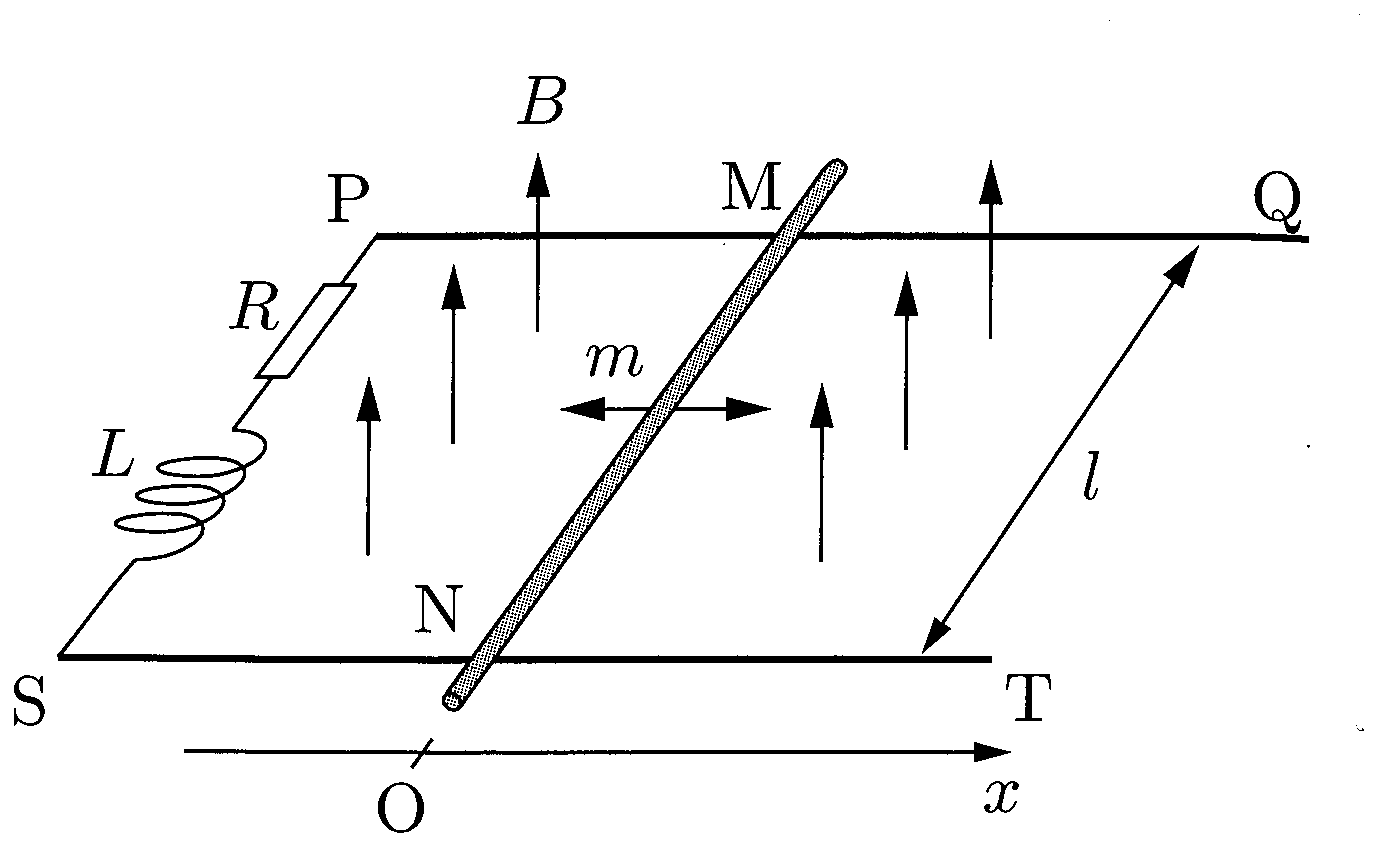
\includegraphics[keepaspectratio,width=60mm]{fig/n32_p130_zu.png}
\end{zuright}
レールと導体棒の抵抗およびそれらの間の接触抵抗は無視でき，また，電気抵抗およびインダクタンスは図の$\mathrm{R}$，$\mathrm{L}$によるもの以外は無視できるものとする．今，$\mathrm{MN}$に外力を加えて，$\mathrm{MN}$を時刻$t\U{s}$に対して$x=a\sin\omega t\U{m}$の式にしたがって$x$軸方向に単振動させた．これについて以下の設問に答えよ．特に断りのない限りは時刻$t$における瞬時値を答えよ．
\begin{komon}
\ko{1} 回路に誘起される起電力$V(t)\U{V}$を求めよ．ただし，$\mathrm{M}\to\mathrm{N}$の向きを起電力の正の向きとする．微分公式$\dfrac{d}{dt}(\sin\omega t)=\omega\cos\omega t$を利用してよい．
\ko{2} 回路に流れる電流$I(t)\U{A}$を式で表せ．ただし，$\mathrm{M}\to\mathrm{N}$の向きを電流の正の向きとする．
\ko{3} 導体棒を単振動させるために加えている外力$F(t)\U{N}$を求めよ．ただし，$+x$の向きを力の正の向きとする．微分公式$\dfrac{d}{dt}(\cos\omega t)=-\omega\sin\omega t$を利用してよい．
\end{komon}

\Mon{リサジュー図形}

\hspace{1zw}電圧の最大値が$V_0\U{V}$，周波数が$f\U{Hz}$（角周波数$\omega=2\pi f\U{rad/s}$）の交流電源に，図1のように抵抗（抵抗値$R\U{\Omega}$）とコイル（自己インダクタンス$L\U{H}$）を直列につなぎ，端子$\mathrm{A}$，$\mathrm{B}$，$\mathrm{C}$をつける．図2はブラウン管の概略図である．
\begin{center}
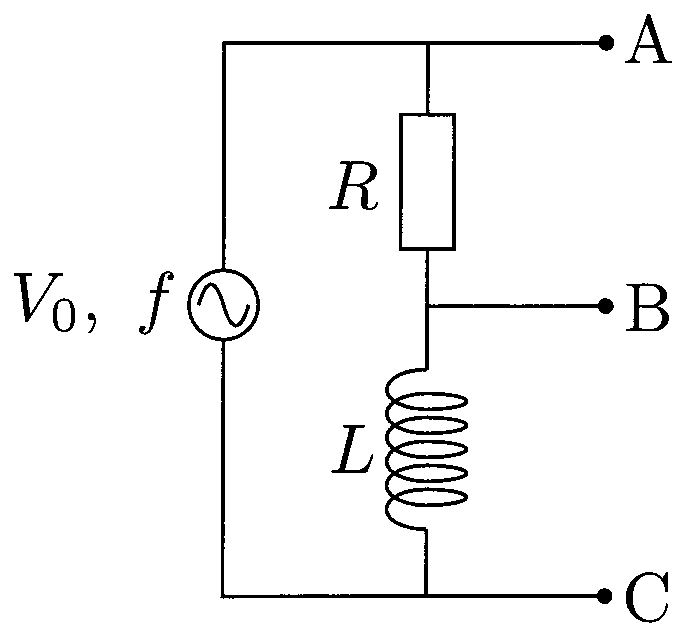
\includegraphics[keepaspectratio,width=36mm]{fig/n32_p131_zu1.png}\hspace{8mm}%
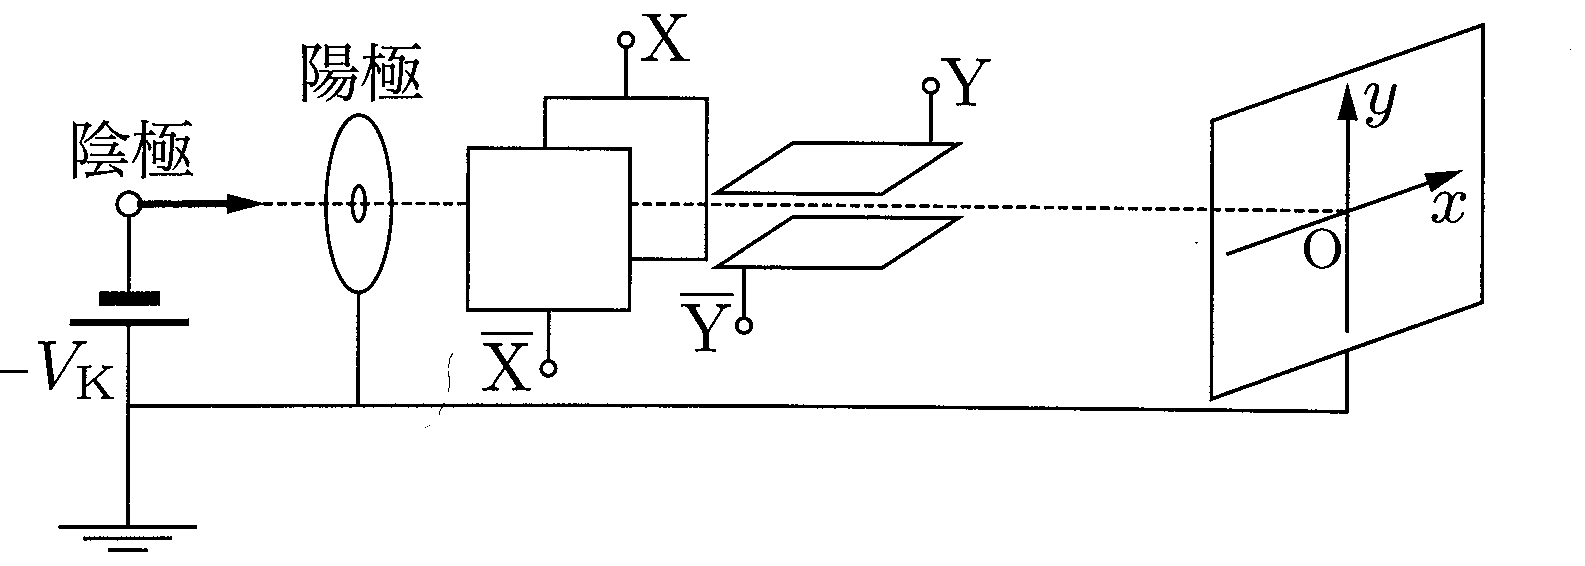
\includegraphics[keepaspectratio,width=90mm]{fig/n32_p131_zu2.png}\\
{\small 図1}\hspace{60mm}{\small 図2}
\end{center}
\hspace{1zw}電位$-V_{\mathrm{K}}\U{V}$（ただし$V_{\mathrm{K}}>0$である）の陰極から初速$0$で出た電子は，接地された陽極の小孔を通過するまでの間に加速された後，端子をつけた等面積の4枚の正方形極板$\mathrm{X}$，$\overline{\mathrm{X}}$，$\mathrm{Y}$，$\overline{\mathrm{Y}}$の間を通り，蛍光面に当たって輝点を生じる．蛍光面上に，陰極と陽極の小孔を結ぶ直線上の点を原点として直交する$x$，$y$軸を取り，面上の位置を表すものとする．一組の極板$\mathrm{X}$，$\overline{\mathrm{X}}$はそれらの面がともに$x$軸方向に垂直に向かい合って配置され，$\mathrm{X}$，$\overline{\mathrm{X}}$と同じ間隔で向かい合う他の一組の極板$\mathrm{Y}$，$\overline{\mathrm{Y}}$はそれらの面が$y$軸方向に垂直に配置されている．図1の回路に極板をつなぐことによって生じる回路の電流の変化は無視してよく，また，極板の辺の長さや二組の極板間の距離に比べて蛍光面から極板までの距離は十分に大きい．また，$V_{\mathrm{K}}$は$V_0$より十分に大きい．さらに，加速された電子は速く，各電子が二組の極板を通過する時間内での交流電圧の変化は考えなくてよいものとする．
\par
\hspace{1zw}今，$\mathrm{X}$に$\mathrm{A}$を，$\overline{\mathrm{X}}$に$\mathrm{B}$をつなぎ，$\mathrm{Y}$，$\overline{\mathrm{Y}}$を接地すると，蛍光面の$x$軸上の直線部分$-a\leqq x\leqq a\U{m}$が光る．これは次のようにして説明される．$\mathrm{X}$に$\mathrm{A}$を，$\overline{\mathrm{X}}$に$\mathrm{B}$をつなぐと$\mathrm{X}$，$\overline{\mathrm{X}}$に対して抵抗にかかる交流電圧がかかることになる．抵抗にかかる交流電圧は時間変化していること，および$\mathrm{X}$，$\overline{\mathrm{X}}$間の電場の強さと電子線の偏向の度合（$x$軸方向にどれだけねじまげられるか）が比例することに注意すると，$\mathrm{X}$，$\overline{\mathrm{X}}$にかかる電圧が$-V_{R0}\U{V}\sim +V_{R0}\U{V}$の範囲で時間変化するとそれによって電子の蛍光面への到達点が$-a\leqq x\leqq a\U{m}$の範囲で変化する．蛍光面の光は残像が残ること，および交流電圧の周波数は一般に$50\sim 60\U{Hz}$であるため，光る点の$-a\leqq x\leqq a\U{m}$の範囲での振動を目で追い切ることができず，$-a\leqq x\leqq a\U{m}$の範囲のすべての点が同時に光っているように見える．
\par
\hspace{1zw}以上のこと，および$\mathrm{AB}$間の電圧ならびに$\mathrm{BC}$間の電圧には位相差があることに注意して，以下の設問に述べる操作をしたそれぞれの場合について，蛍光面上のどの部分が光るかを答え，その理由も示せ．
\begin{komon}
\ko{1} $\mathrm{X}$に$\mathrm{B}$を，$\overline{\mathrm{X}}$に$\mathrm{C}$をつなぎ，$\mathrm{Y}$，$\overline{\mathrm{Y}}$を接地する．
\ko{2} $\mathrm{X}$に$\mathrm{A}$を，$\overline{\mathrm{X}}$と$\mathrm{Y}$に$\mathrm{B}$を，$\overline{\mathrm{Y}}$に$\mathrm{C}$をつなぐ．
\ko{3} (2)において，交流電源の周波数を$\dfrac{1}{3}f\U{Hz}$にする．
\end{komon}

\newpage

%%%%%%%%%%%%%%%%%%%%  解答  %%%%%%%%%%%%%%%%%%%%
\KaiTitle{第32回　交流回路・共振と電磁波}
\setlength{\columnseprule}{0.4pt}
\begin{multicols}{2}
\raggedcolumns

\Rank{A問題}
\MonN{120}{基本公式の確認}\par\nopagebreak
\begin{sisin}
直列回路のインピーダンスの式$Z=\sqrt{R^2+\bigl(\omega L-\frac{1}{\omega C}\bigr)^2}$を利用して答えよう．2つの素子からなる直列回路なら，無い素子の項を消せばよい．

インピーダンスは電圧・電流の最大値（あるいは実効値）の比にすぎないから，インピーダンスで分かるのは電流と電圧の大きさの関係だけである．直流回路の抵抗と同じだと錯覚しがちだが，交流回路の電圧・電流には位相があり，その差についても考える必要がある．
\end{sisin}
\KaiHead
\begin{komon}
\ko{1} \[\begin{aligned}Z&=\sqrt{R^2+\Bigl(2\pi fL-\frac{1}{2\pi fC}\Bigr)^2}\\&=\sqrt{5^2+(112-100)^2}=1.30\times 10\U{\Omega}\end{aligned}\]
       \hspace*{\fill}$\cdots$(答)
\ko{2} $\dfrac{1}{2\pi fC}=\dfrac{1}{2\pi\cdot 50\cdot\frac{10^4\times 10^{-6}}{7\pi}}=7$なので
       \[Z=\sqrt{24^2+7^2}=2.50\times 10\U{\Omega}\Ans\]
\ko{3} $2\pi fL=2\pi\cdot 50\cdot\dfrac{100\times 10^{-3}}{\pi}=10$なので
       \[Z=\sqrt{10^2+10^2}\fallingdotseq 14.1\U{\Omega}\Ans\]
\end{komon}

\MonN{121}{電磁波の分類}\par\nopagebreak
\begin{sisin}
電磁波については，\MARU{1}何が電磁波なのか，\MARU{2}波長のおおざっぱな大小関係，\MARU{3}可視光の波長範囲（およそ$380\sim 780\U{nm}$），\MARU{4}光の色の並び方を覚えておくこと（32.5）．
\end{sisin}
\KaiHead
(1)〜(6)はすべて電磁波である．波長の長いものから並べると
\[(5)>(6)>(4)>(1)>(2)>(3)\Ans\]
\begin{chuu}
まず可視光のすぐ両脇に赤外線，紫外線がくる（赤色光，紫色光のすぐ外側という意味で名前がついている．赤の方が波長が長い）．X線は透過力が高く，紫外線よりさらに短波長側に来る（波長が短いほどエネルギーが大きい）．ラジオやテレビは波長の長い電磁波を使う．ラジオ波の方が波長が長く，回折しやすい．
\end{chuu}

\Rank{B問題}
\MonN{122}{RL直列回路}\par\nopagebreak
\begin{sisin}
交流回路の問題は，キルヒホッフの第二法則をベクトル図で表し，その図をもとに考えていくのが基本である（32.2）．直列接続では，\MARU{1}電流が共通なので電流の最大値・位相を仮定し，\MARU{2}それをもとに各素子の電圧の最大値・位相を求め，\MARU{3}第二法則をベクトル図で表す．

与えられている電圧値は実効値であり，実際の電圧は時間変動している．(3)でも，{\gtfamily （電源電圧の実効値）$\neq$（抵抗の電圧の実効値）$+$（コイルの電圧の実効値）}であることに注意せよ．位相が与えられていなくても位相が存在しないわけではない．扱いやすさから，電流の位相を$\omega t$と仮定するとよい．
\end{sisin}
\KaiHead
電源電圧の最大値は$V_0=100\sqrt{2}\U{V}$，角周波数は$\omega=2\pi f=200\pi\U{rad/s}$である．
\begin{center}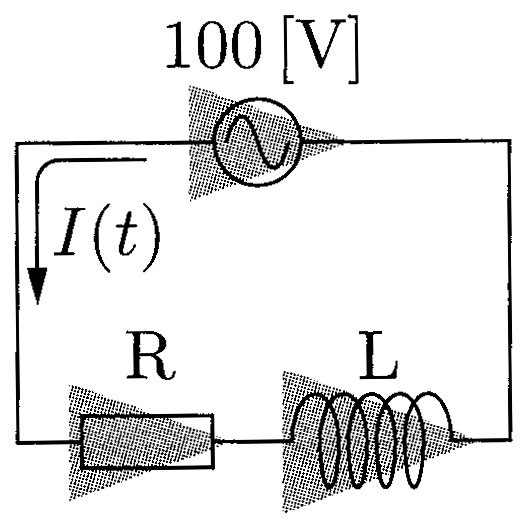
\includegraphics[keepaspectratio,width=34mm]{fig/n32_a122_zu.png}\end{center}
\begin{komon}
\ko{1} 流れる電流を$I(t)=I_0\sin\omega t$と仮定すると，$V_R(t)=RI_0\sin\omega t$，$V_L(t)=\omega LI_0\sin\bigl(\omega t+\frac{\pi}{2}\bigr)$であり，時刻$t$において抵抗およびコイルにかかる電圧は次図のベクトルの$y$軸投影で表される．
       \begin{center}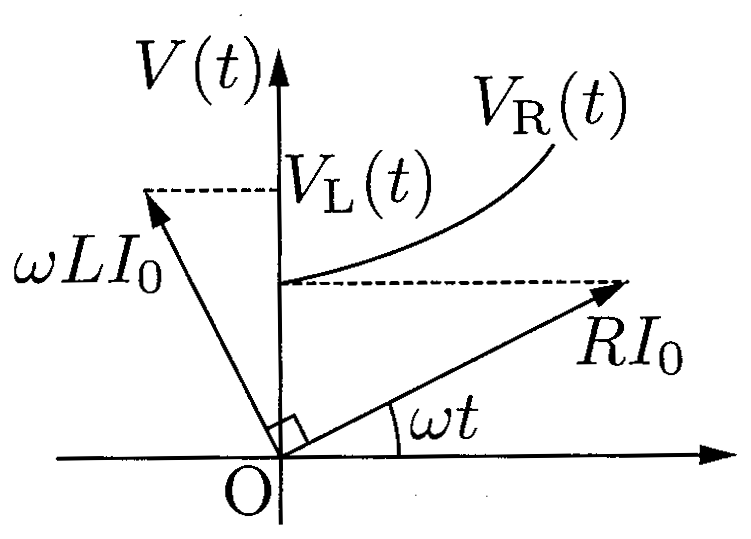
\includegraphics[keepaspectratio,width=44mm]{fig/n32_a122_vec1.png}\end{center}
       キルヒホッフの第二法則より，その和（二つのベクトルの和の$y$軸投影）が電源電圧である．
       \begin{center}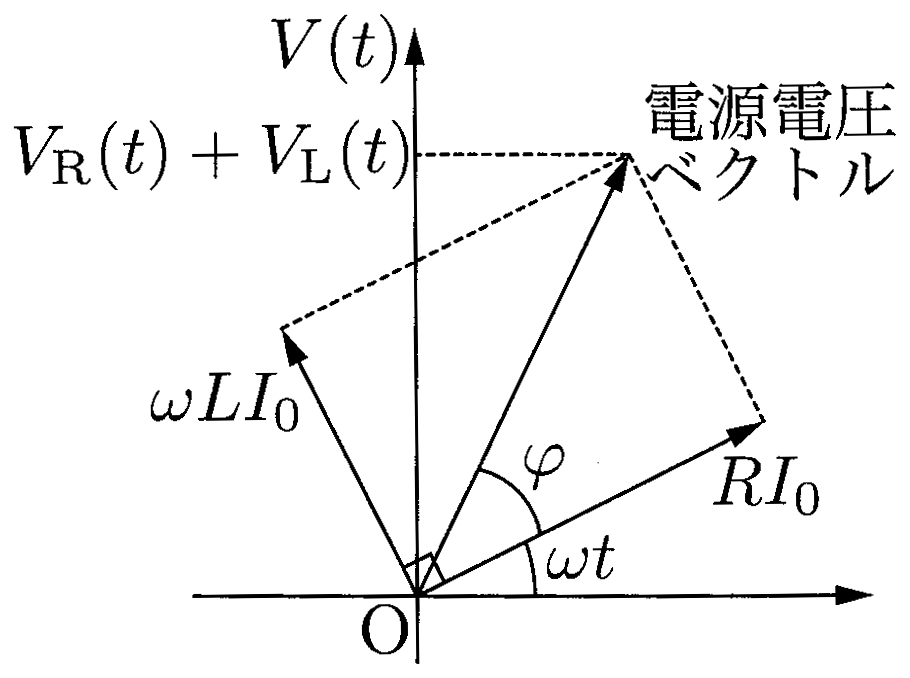
\includegraphics[keepaspectratio,width=48mm]{fig/n32_a122_vec2.png}\end{center}
       よって$V_0=\sqrt{(RI_0)^2+(\omega LI_0)^2}$．値を代入して
       \[100\sqrt{2}=\sqrt{(100I_0)^2+(200\pi\cdot 0.159\cdot I_0)^2}\]
       これを解いて$I_0\fallingdotseq 1.00\U{A}$．ゆえに実効値は
       \[\frac{I_0}{\sqrt{2}}\fallingdotseq 0.707\U{A}\Ans\]
\ko{2} 前図で電源電圧ベクトルと抵抗の電圧ベクトルのなす角を$\varphi$とすると，電源電圧は$V(t)=V_0\sin(\omega t+\varphi)$で，電流の位相は電源電圧より$\varphi$遅れる．$\tan\varphi=\dfrac{\omega L}{R}=1.00$より$\varphi=\dfrac{\pi}{4}$．よって位相差は
       \[-\frac{\pi}{4}\U{rad}\Ans\]
\ko{3} $V_{R0}=RI_0=100\U{V}$，$V_{L0}=\omega LI_0=100\U{V}$なので，実効値はどちらも
       \[\frac{100}{\sqrt{2}}\fallingdotseq 70.7\U{V}\Ans\]
       \begin{chuu}
       素子の電圧の実効値の和$70.7+70.7$は電源電圧の実効値$100\U{V}$にならない．実効値については直流と同じ感覚で足してはならない．
       \end{chuu}
\ko{4} \[Z=\frac{V_0}{I_0}=\frac{100\sqrt{2}}{1.00}\fallingdotseq 141\U{\Omega}\Ans\]
\end{komon}

\MonN{123}{RC直列回路}\par\nopagebreak
\begin{sisin}
攻め方は前問と同じで，ベクトル図を用いて回路に成り立つ関係式を求め，それをもとに各設問に答えていく．(2)〜(4)で，コンデンサーの電圧が$8.0\U{V}$だから抵抗の電圧は$2.0\U{V}$，などとは考えないこと．与えられているのは実効値であり，実効値でキルヒホッフの第二法則を考えてはならない．
\end{sisin}
\KaiHead
$V_0=10.0\sqrt{2}\U{V}$，$\omega=2\pi f_0$である．
\begin{komon}
\ko{1} $\mathrm{C}_2$の容量を$C$とし，電流を$I(t)=I_0\sin\omega t$とおく．$\mathrm{C}_1$，$\mathrm{C}_2$の電圧はどちらも電流より$\dfrac{\pi}{2}$遅れた同じ向きのベクトルになる．
       \begin{center}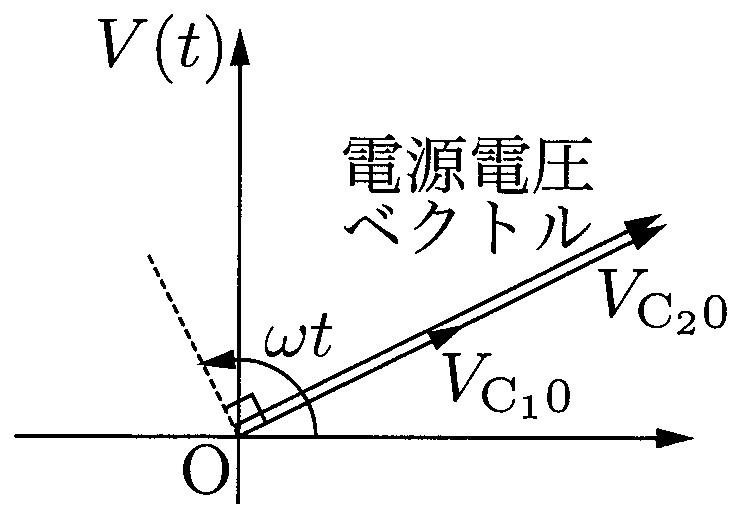
\includegraphics[keepaspectratio,width=44mm]{fig/n32_a123_vec1.png}\end{center}
       よって
       \[\frac{I_0}{\omega C}+\frac{I_0}{\omega\cdot 0.10\times 10^{-6}}=10.0\sqrt{2}\]
       \[\frac{I_0}{\omega C}=8.0\sqrt{2}\]
       以上2式より
       \[C=0.025\times 10^{-6}\U{F}=0.025\U{\mu F}\Ans\]
\ko{2} 図2の回路で電流を$I^\prime(t)=I_0^\prime\sin\omega t$とおくと，抵抗の電圧は電流と同じ向き，$\mathrm{C}_2$の電圧は$\dfrac{\pi}{2}$遅れた向きで，両者は直交する．
       \begin{center}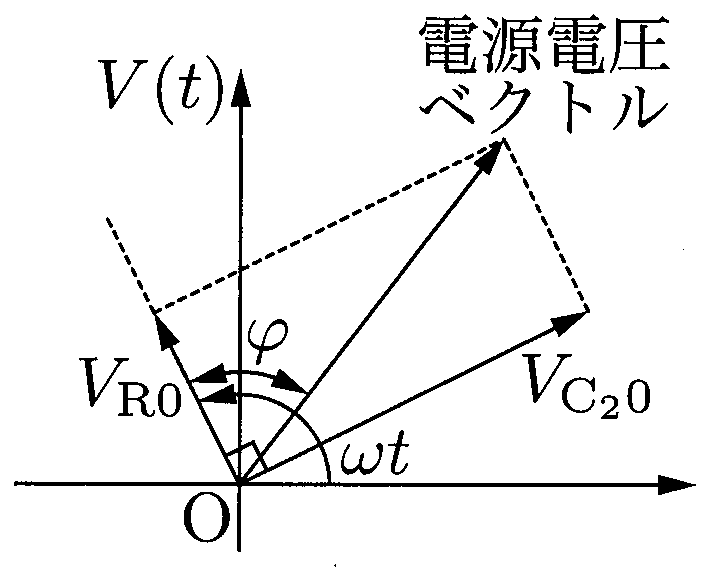
\includegraphics[keepaspectratio,width=44mm]{fig/n32_a123_vec2.png}\end{center}
       よって
       \[\sqrt{(RI_0^\prime)^2+\Bigl(\frac{I_0^\prime}{\omega C}\Bigr)^2}=10.0\sqrt{2}\]
       \[\frac{I_0^\prime}{\omega C}=8.0\sqrt{2}\]
       抵抗の電圧の実効値は
       \[\frac{RI_0^\prime}{\sqrt{2}}=\sqrt{10.0^2-8.0^2}=6.0\U{V}\Ans\]
\ko{3} % 原本は分母を 3×10^3 と書いていた（問題文は 30 kΩ．答の値は正しい）．
       \[\frac{I_0^\prime}{\sqrt{2}}=\frac{6.0}{30\times 10^3}=2.0\times 10^{-4}\U{A}\Ans\]
\ko{4} \[Z=\frac{10.0}{2.0\times 10^{-4}}=5.0\times 10^4\U{\Omega}\Ans\]
\ko{5} $\dfrac{I_0^\prime}{\omega C}=8.0\sqrt{2}$と$C=0.025\times 10^{-6}\U{F}$より
       \[\omega=\frac{2.0\times 10^{-4}}{8.0\times 0.025\times 10^{-6}}=1.0\times 10^3\U{rad/s}\]
       \[f_0=\frac{1.0\times 10^3}{2\times 3.14}\fallingdotseq 1.6\times 10^2\U{Hz}\Ans\]
\end{komon}

\MonN[\Sitei]{124}{RLC直列共振回路}\par\nopagebreak
\begin{sisin}
直列共振の周波数は$f=\dfrac{1}{2\pi\sqrt{LC}}$という結果式で求められるが，このとき回路でどういうことが起こり，どういう特徴があるのかをしっかり押さえておくこと（32.3）．

ベクトル図全体を$\dfrac{1}{\sqrt{2}}$倍しても角度は保たれ，長さが実効値になる．電流・電圧が実効値で与えられているときは，実効値でベクトル図を描いてよい（32.1）．
\end{sisin}
\KaiHead
\begin{komon}
\ko{1} 電流の実効値を$\overline{I}$とすると，各素子の電圧の実効値は$\overline{V_R}=R\overline{I}$，$\overline{V_L}=\omega L\overline{I}$，$\overline{V_C}=\dfrac{\overline{I}}{\omega C}$であり，ベクトル図は次のようになる．
       \begin{center}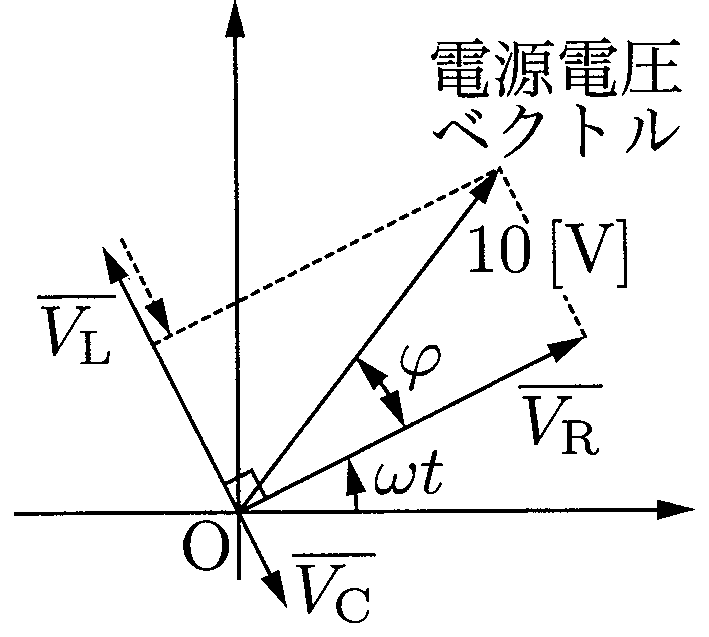
\includegraphics[keepaspectratio,width=40mm]{fig/n32_a124_vec1.png}\end{center}
       $10^2=\overline{V_R}^2+(\overline{V_L}-\overline{V_C})^2$より
       \[\overline{I}=\frac{10}{\sqrt{R^2+\bigl(\omega L-\frac{1}{\omega C}\bigr)^2}}\]
       共振しているときは$\overline{V_L}=\overline{V_C}$，すなわち$\omega=\dfrac{1}{\sqrt{LC}}$のときなので，
       \[f=\frac{1}{2\pi\sqrt{0.40\times 1.0\times 10^{-5}}}\fallingdotseq 8.0\times 10\U{Hz}\]
       \hspace*{\fill}$\cdots$(答)
\ko{2} $\omega=\dfrac{1}{\sqrt{LC}}$のとき$\overline{I}$の分母が最小になるので，{\gtfamily 回路に流れる電流の実効値が最大になる}．\Ans
       また$\overline{V_L}=\overline{V_C}$で，コイルとコンデンサーの電圧が打ち消し合うので，電源電圧がそのまま抵抗にかかる．
       \begin{center}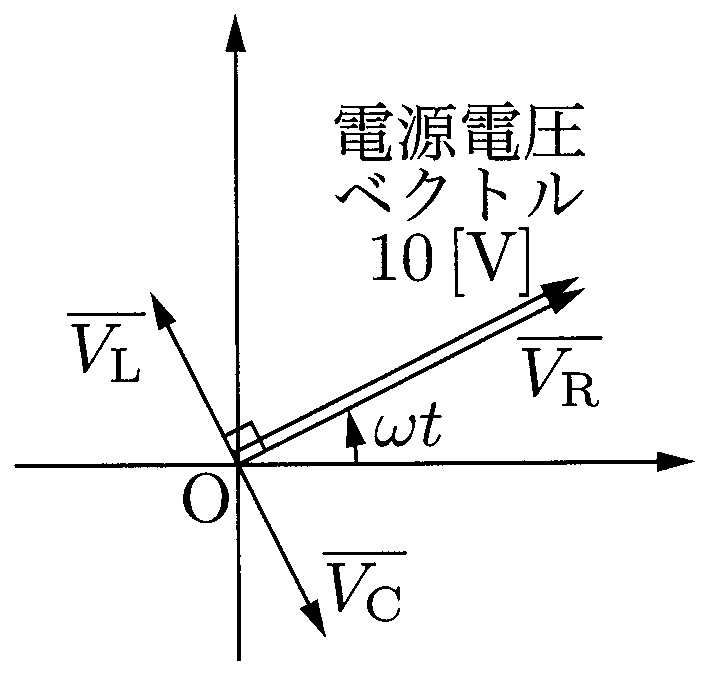
\includegraphics[keepaspectratio,width=40mm]{fig/n32_a124_vec2.png}\end{center}
       コイル・コンデンサーでは電力が消費されないので，{\gtfamily 回路での消費電力（$R\overline{I}^2$）が最大になっている}．\Ans
\ko{3} 共振時の角周波数は$\omega=\dfrac{1}{\sqrt{LC}}=500\U{rad/s}$．コイルの電圧が$100\U{V}$のとき$100=500\times 0.40\times\overline{I}$より$\overline{I}=5.0\times 10^{-1}\U{A}$．抵抗には電源電圧$10\U{V}$がそのままかかるので
       \[R=\frac{10}{5.0\times 10^{-1}}=20\U{\Omega}\Ans\]
\ko{4} 共振しているので
       \[\overline{V_C}=\overline{V_L}=100\U{V}\Ans\]
\end{komon}

\MonN{125}{電流・電圧グラフの読み取り}\par\nopagebreak
\begin{sisin}
グラフの読み取りに注意．「$I(t)$の方が$V(t)$のグラフより右へ進んでいるから，$I(t)$の位相の方が進んでいる」と考えるのは誤りである．最大値を取る時刻に着目すれば，$I(t)$の方が最大値を取る時刻が遅れている，すなわち位相が遅れていると判断できる．
本問もベクトル図を描いて考え，それから設問を順番に解いていくとよい．グラフからは最大値が読み取れるので，ベクトルの長さは最大値で取るとよいだろう．
% 原本は「B問題［34］と同様に」（旧回の番号）．
\end{sisin}
\KaiHead
\begin{komon}
\ko{1} グラフより$V_0=141\U{V}$，周期$T=0.02\U{s}$なので，$f=\dfrac{1}{T}=50\U{Hz}$，$\omega=100\pi\U{rad/s}$．よって
       \[f=50\U{Hz},\qquad\overline{V}=\frac{V_0}{\sqrt{2}}\fallingdotseq 100\U{V}\Ans\]
\ko{2} グラフより
       \[\begin{aligned}I(t)&=2.82\sin\{100\pi(t-0.0025)\}\\&=2.82\sin\Bigl(\omega t-\frac{\pi}{4}\Bigr)\\V(t)&=141\sin\omega t\end{aligned}\]
       抵抗の電圧は電流と同位相なので，ベクトル図は次のようになる．
       \begin{center}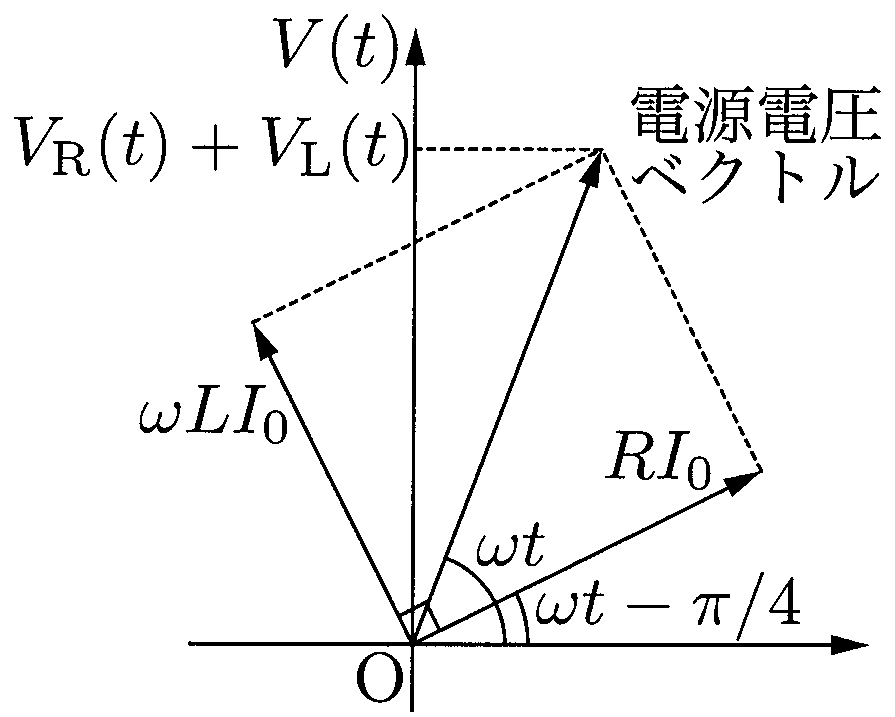
\includegraphics[keepaspectratio,width=46mm]{fig/n32_a125_vec.png}\end{center}
       幾何学的関係から
       \[\frac{\omega LI_0}{RI_0}=\tan\frac{\pi}{4}\quad\cdots\text{\MARU{1}}\]
       \[(\omega LI_0)^2+(RI_0)^2=V_0^2\quad\cdots\text{\MARU{2}}\]
       \MARU{1}より$\omega LI_0=RI_0$なので\MARU{2}は$2(RI_0)^2=V_0^2$．$I_0=2.82$，$V_0=141$を代入して
       \[R=\frac{50}{\sqrt{2}}\fallingdotseq 35.3\U{\Omega}\Ans\]
\ko{3} $\omega L=R$より
       \[L=\frac{R}{\omega}=\frac{1}{100\pi}\cdot\frac{50}{\sqrt{2}}\fallingdotseq 1.13\times 10^{-1}\U{H}\Ans\]
\end{komon}

\MonN[\Sitei]{126}{並列共振回路}\par\nopagebreak
\begin{sisin}
並列・直列が入り乱れた交流回路では，キルヒホッフの第二法則をどう利用すればよいかをまず考えよ．並列接続なら電圧が共通，直列接続なら電流が共通である．本問では，コイルとコンデンサーにかかる電圧（$\mathrm{bd}$間の電圧）を仮定すれば，\MARU{1}コイル・コンデンサーの電流が分かり，\MARU{2}それをもとに抵抗の電流が分かり，\MARU{3}抵抗の電圧が分かり，\MARU{4}回路の第二法則を用いることができる．「直列なら電流を仮定する」という紋切り型ではなく，「何を仮定すれば第二法則を適用できるか」を考えよ（32.4）．
\end{sisin}
\KaiHead
\begin{komon}
\ko{1} $\omega=2\pi f$とおき，$\mathrm{d}$に対する$\mathrm{b}$の電位を$V_{\mathrm{bd}}(t)=V_{0\mathrm{bd}}\sin(\omega t-\varphi)$と仮定する．さらに$\omega C>\dfrac{1}{\omega L}$と仮定する．コイル，コンデンサーを下向きに流れる電流$I_C(t)$，$I_L(t)$は逆向きのベクトルになる．$\mathrm{b}$点で第一法則を用いると抵抗の電流は$I_C+I_L$で，抵抗の電圧降下は$R(I_C+I_L)$と表せる．
       \begin{center}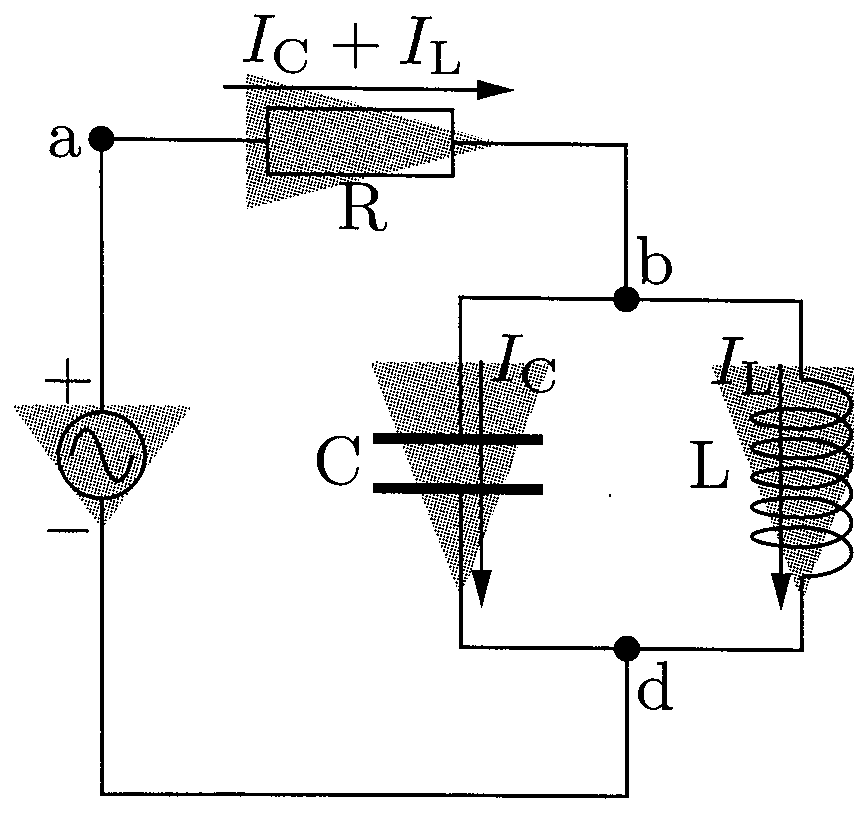
\includegraphics[keepaspectratio,width=40mm]{fig/n32_a126_zu.png}\end{center}
       第二法則より，抵抗の電圧と$\mathrm{bd}$間の電圧の和が電源電圧に等しいので，次図のような関係が得られる．
       \begin{center}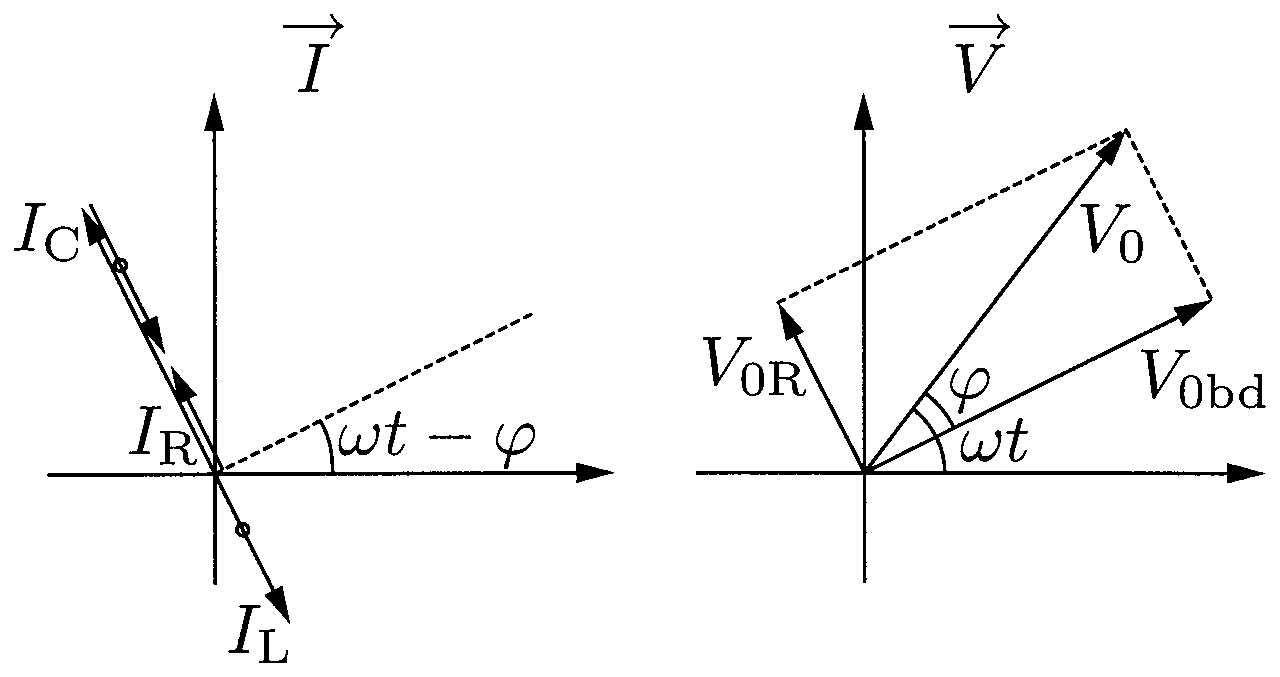
\includegraphics[keepaspectratio,width=58mm]{fig/n32_a126_vec.png}\end{center}
       抵抗を流れる電流の最大値は
       \[I_{0R}=I_{0C}-I_{0L}=\Bigl(\omega C-\frac{1}{\omega L}\Bigr)V_{0\mathrm{bd}}\]
       $\omega C=\dfrac{1}{\omega L}$のとき抵抗を流れる電流の最大値が$0$になるので，求める$f_0$は$(2\pi f_0)C=\dfrac{1}{(2\pi f_0)L}$より
       \[f_0=\frac{1}{2\pi\sqrt{LC}}\U{Hz}\Ans\]
       \begin{bsHosoku}{参考}
       このときの状態も共振といい（並列共振），電源から電流が全く出ていかず，LC 部分で電気振動が起こるのみとなる．よって電源の消費電力は$0$である（直列共振と周波数は同じだが，消費電力の最大・最小が合致しない点に十分注意）．
       \end{bsHosoku}
\ko{2} ベクトル図より，抵抗の電圧の最大値は$V_{0R}=RI_{0R}=R\bigl(\omega C-\frac{1}{\omega L}\bigr)V_{0\mathrm{bd}}$で，三平方の定理より$V_{0R}^2+V_{0\mathrm{bd}}^2=V_0^2$．以上より
       \[V_{0\mathrm{bd}}=\frac{V_0}{\sqrt{1+R^2\bigl(\omega C-\frac{1}{\omega L}\bigr)^2}}\]
       $\omega\to\infty$の極限で$V_{0\mathrm{bd}}\to 0$なので$V_{0R}=V_0$．よって抵抗を流れる電流の実効値は
       \[\overline{I_R}=\frac{V_0}{\sqrt{2}R}\U{A}\Ans\]
       \begin{chuu}
       $I_{0R}=\bigl(\omega C-\frac{1}{\omega L}\bigr)V_{0\mathrm{bd}}$の式で$\omega\to\infty$とすると$\infty\times 0$の不定形になるので，この式から直接極限を取ってはいけない．
       \end{chuu}
       \begin{bsHosoku}{参考}
       $X_C=\dfrac{1}{\omega C}$，$X_L=\omega L$より，$\omega\to\infty$ではコイルは電流を通さない（断線と同じ），コンデンサーは電流をそのまま通す（ただの導線と同じ）．よって回路は次図と同じになり，$\overline{I_R}=\dfrac{V_0}{\sqrt{2}R}$となる（32.4）．この性質を使えば，高周波だけ・低周波だけを通すフィルターを作ることができる．
       \begin{center}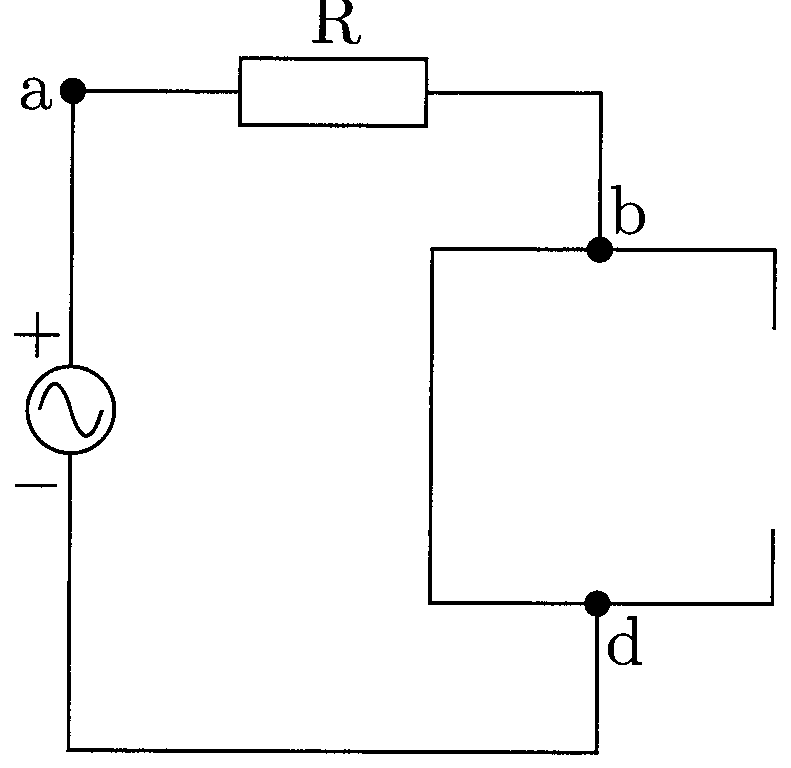
\includegraphics[keepaspectratio,width=36mm]{fig/n32_a126_lim.png}\end{center}
       \end{bsHosoku}
\end{komon}

\MonN{127}{複雑な交流回路}\par\nopagebreak
\begin{sisin}
考え方，方針は前問と全く同様である．位相については触れられていないが，ベクトル図を用いて位相についても考えなければならない．(2)はベクトル図が直角三角形になっていないことに注意．電流ベクトル図と電圧ベクトル図をよく見比べて角度を移しながら考えること．
\end{sisin}
\KaiHead
各素子の電圧・電流を$V_1\sim V_3$，$V_C$，$I_1\sim I_3$，$I_C$で表し，上付きのバーで実効値を表す．ベクトルの長さは実効値で示す．
\begin{komon}
\ko{1} $\mathrm{R}_2$の電流の位相を$\omega t$と仮定する．$\mathrm{R}_2$の電圧とコンデンサーの電圧の和が$\mathrm{R}_3$の電圧であるから，ベクトル図で考えると次図のようになる．
       \begin{center}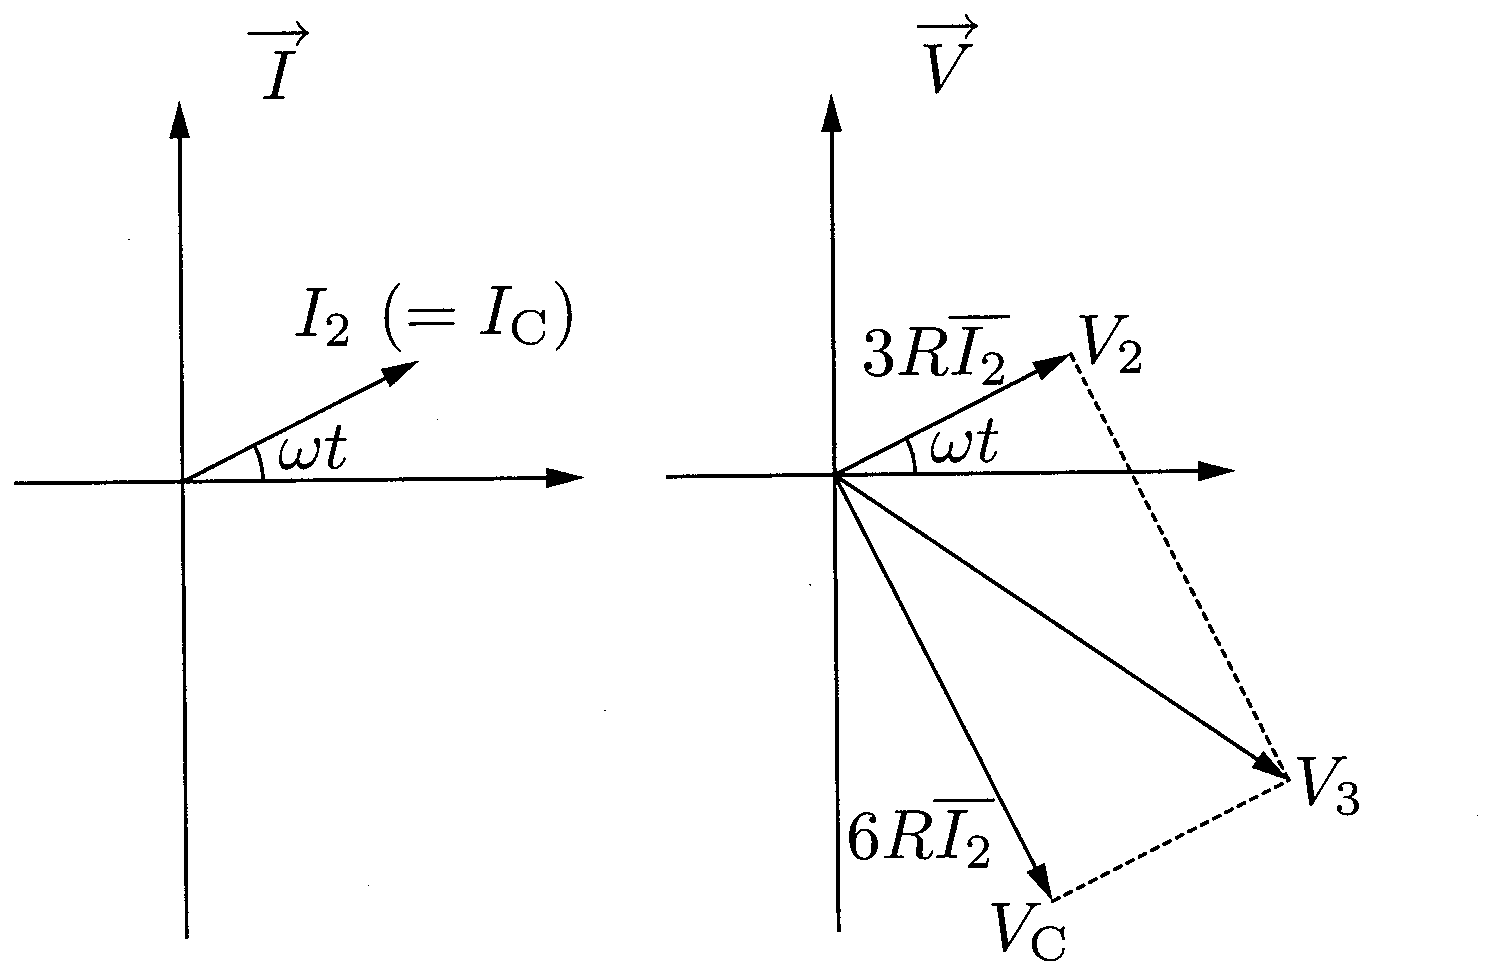
\includegraphics[keepaspectratio,width=60mm]{fig/n32_a127_vec1.png}\end{center}
       よって
       \[\begin{aligned}\overline{V_3}&=\sqrt{(3R\overline{I_2})^2+(6R\overline{I_2})^2}\\&=3\sqrt{5}R\overline{I_2}\U{V}\end{aligned}\]
       \hspace*{\fill}$\cdots$(答)
\ko{2} $\mathrm{R}_3$の電流は$\overline{I_3}=\dfrac{\overline{V_3}}{6R}=\dfrac{\sqrt{5}}{2}\overline{I_2}$で，位相は$V_3$と同じ．$\mathrm{R}_1$の電流は$I_2$と$I_3$のベクトル和である．
       \begin{center}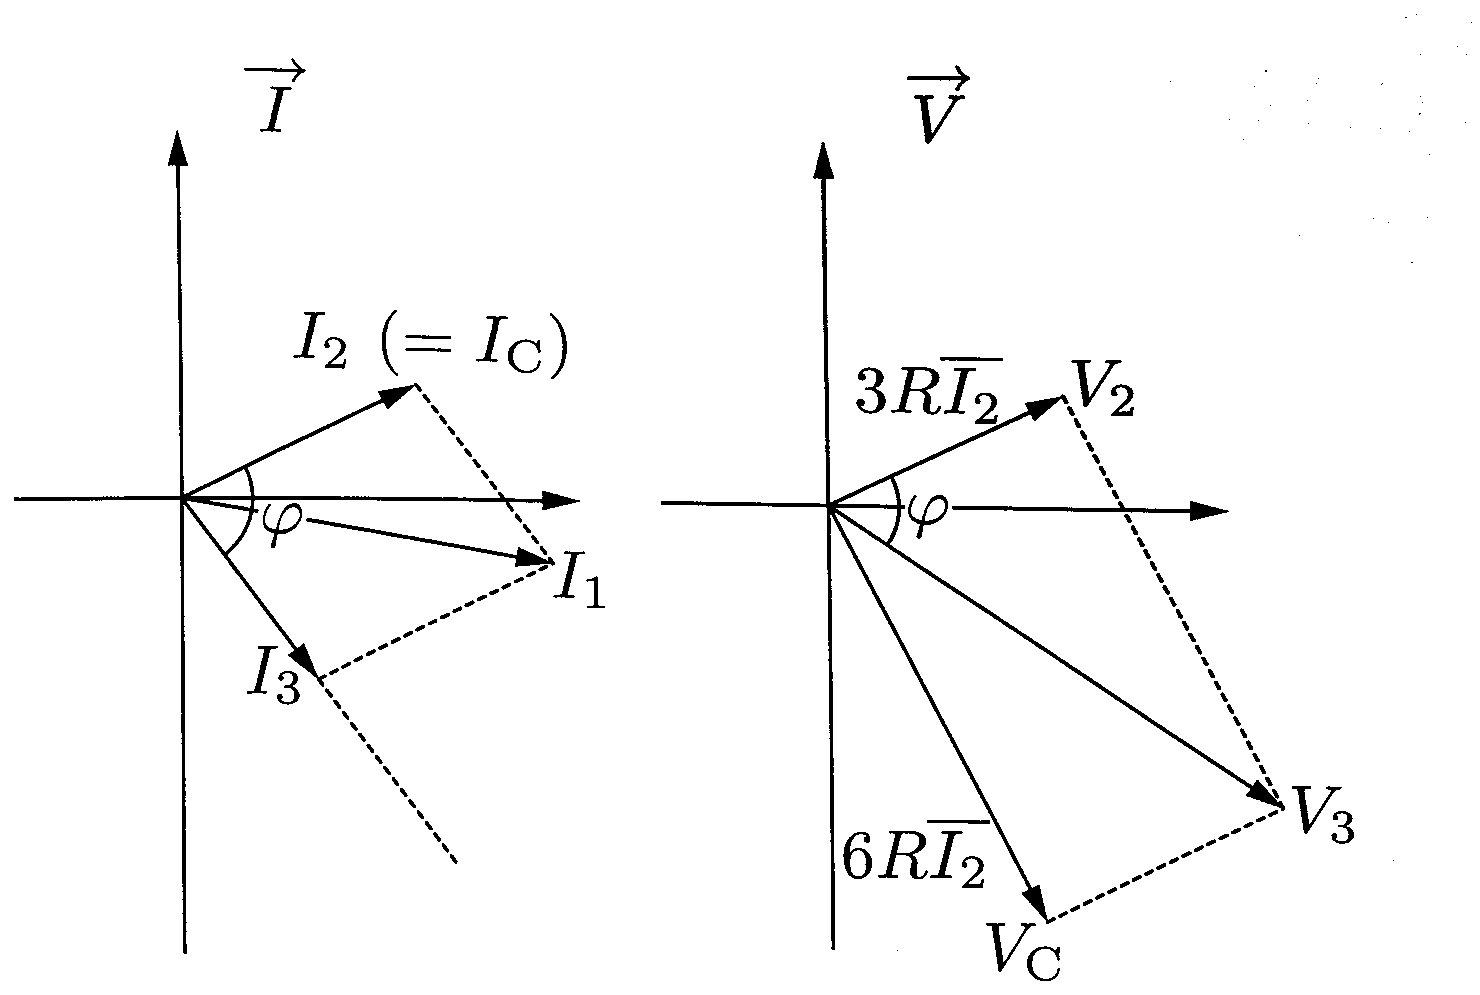
\includegraphics[keepaspectratio,width=60mm]{fig/n32_a127_vec2.png}\end{center}
       電圧ベクトル図より$\cos\varphi=\dfrac{\overline{V_2}}{\overline{V_3}}=\dfrac{1}{\sqrt{5}}$，$\sin\varphi=\dfrac{2}{\sqrt{5}}$．電流ベクトル図の平行四辺形の対角線を求めると
       \[\overline{I_1}^2=(\overline{I_2}+\overline{I_3}\cos\varphi)^2+(\overline{I_3}\sin\varphi)^2\]
       これを解いて
       \[\overline{I_1}=\frac{\sqrt{13}}{2}\overline{I_2}\U{A}\Ans\]
\ko{3} $\mathrm{R}_1$の電圧の実効値は$\overline{V_1}=2R\overline{I_1}=\sqrt{13}R\overline{I_2}$で，位相は$I_1$と同じ．$V_1$と$V_3$のベクトル和の長さが電源電圧の実効値$\overline{V}$になっている．
       \begin{center}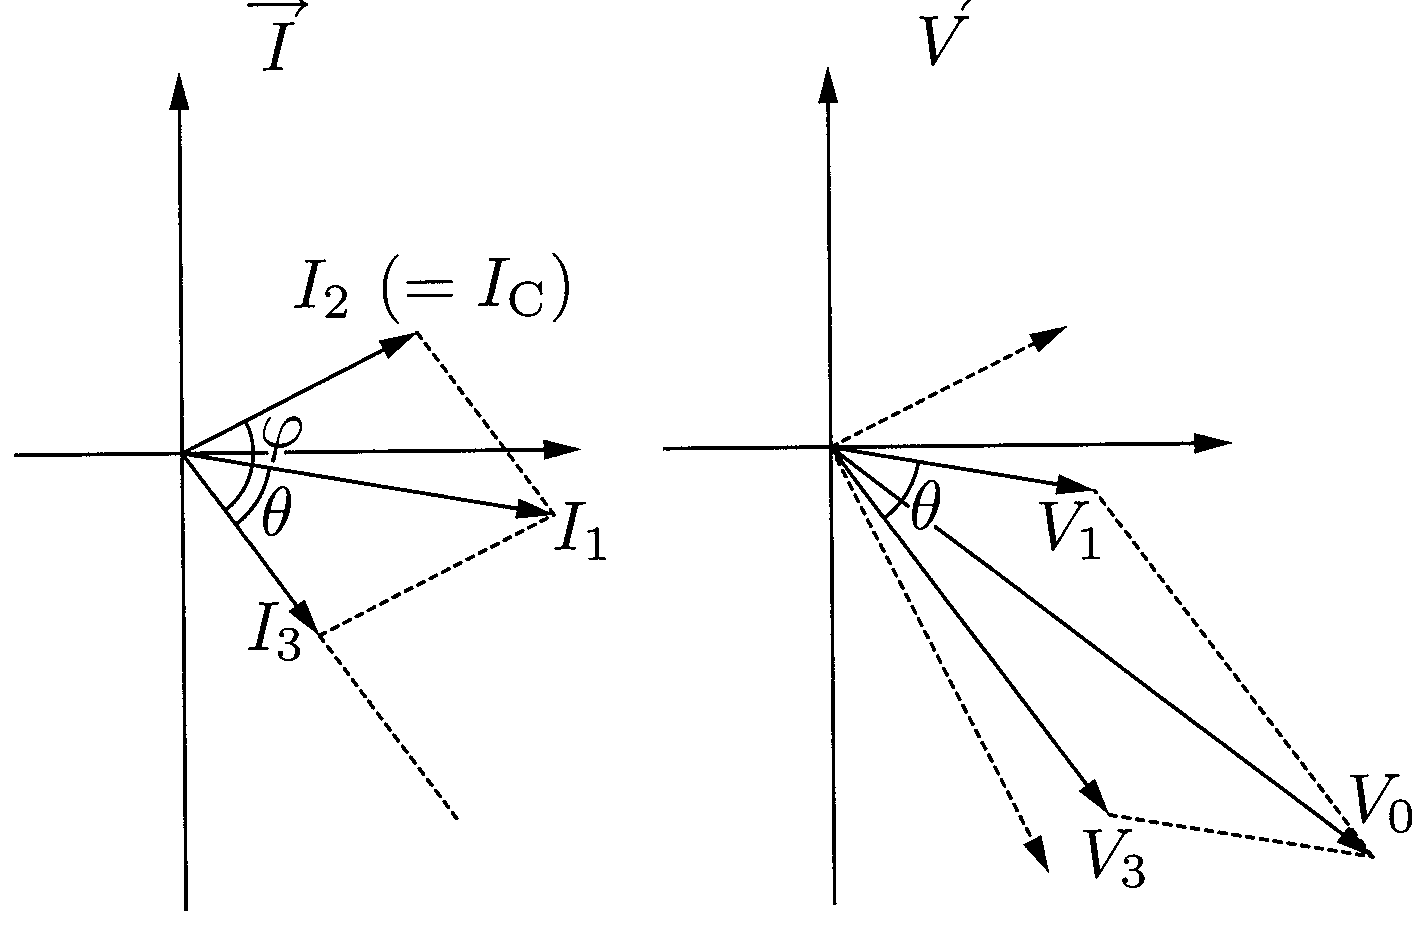
\includegraphics[keepaspectratio,width=60mm]{fig/n32_a127_vec3.png}\end{center}
       電流ベクトル図より$\cos\theta=\dfrac{\overline{I_1}^2+\overline{I_3}^2-\overline{I_2}^2}{2\overline{I_1}\,\overline{I_3}}=\dfrac{7}{\sqrt{65}}$，$\sin\theta=\dfrac{4}{\sqrt{65}}$であり，電圧ベクトル図より
       \[\overline{V}^2=(\overline{V_1}+\overline{V_3}\cos\theta)^2+(\overline{V_3}\sin\theta)^2\]
       これを解いて
       \[\overline{I_2}=\frac{\overline{V}}{10R}\U{A}\Ans\]
\end{komon}

\Rank{C問題}
\MonN{128}{直流・交流回路}\par\nopagebreak
\begin{sisin}
直流回路と交流回路とで素子の振る舞いが違うことを題材にした問題である．直流の場合は十分時間が経つとコイルの誘導起電力は$0$で，ただの導線とみなせる．交流の場合はコイルは誘導リアクタンスを持つ．
% 原本は「コイルは容量リアクタンスを持つ」（誘導リアクタンスの誤り）．
本問では位相は問われず，実効値しか問われていないので，直列インピーダンスの式$Z=\sqrt{R^2+(\omega L)^2}$を使うと楽である．$V_0=ZI_0$の両辺を$\sqrt{2}$で割ると$\overline{V}=Z\overline{I}$となり，実効値の間でも同じ関係が成り立つ．
\end{sisin}
\KaiHead
\begin{komon}
\ko{1} 直流ではゆっくり電圧を変えるので定常状態であり，コイルの誘導起電力は$0$．電圧計は抵抗の電圧そのものを測定しているので，図2(a)より
       \[R=\frac{30}{2.0}=15\U{\Omega}\Ans\]
\ko{2} $\overline{V}=Z\overline{I}$より，図2(b)から
       \[Z=\frac{50}{2.0}=25\U{\Omega}\Ans\]
\ko{3} $\omega=2\pi\times 60\U{rad/s}$，$Z=\sqrt{R^2+(\omega L)^2}$より
       \[L=\frac{\sqrt{Z^2-R^2}}{2\pi\times 60}\fallingdotseq 5.31\times 10^{-2}\U{H}\Ans\]
\end{komon}

\MonN{129}{電磁波の発生}\par\nopagebreak
\begin{sisin}
LC 共振回路を利用して電磁波を発生させる装置，すなわちアンテナの原理を簡単な問題にしたのが本問である（32.5）．(4)は，Aと大地とを一つのコンデンサーのようにみなすと分かりやすい．帯電量の変化により電場が変化する．変化する電場のまわりには磁場ができ，変化する磁場のまわりには電場が作られることを覚えておこう．
\end{sisin}
\KaiHead
\begin{komon}
\ko{1} 電気振動\Ans
\ko{2} $2\pi\sqrt{LC}$\Ans
\ko{3} 相互誘導\Ans
\ko{4} 電場\Ans
\ko{5} 磁場\Ans
\ko{6} 電磁波\Ans
\ko{7} 電流（もしくは電荷でもよい）\Ans
\ko{8} 減衰\Ans
\end{komon}

\MonN{130}{コの字型回路}\par\nopagebreak
\begin{sisin}
コの字型回路で導体棒を単振動させると導体棒上に交流電圧が発生する．抵抗・コイルに流れる交流電流は，交流回路の解法に従って解いていけばよい（第30回の誘導起電力と本回の RL 直列回路の組み合わせ）．
(1)では，まず導体棒の速度$v(t)$を求め，$+x$向きに$v(t)$で動いているとして誘導起電力の向き・大きさを決めればよい．(3)で問われているのは電磁力ではなく外力であることに注意．導体棒は単振動しているので加速度を持つ．運動方程式を立てて$F(t)$を求めよう．
\end{sisin}
\KaiHead
\begin{komon}
\ko{1} $\mathrm{MN}$の速度は$v(t)=\dfrac{dx}{dt}=a\omega\cos\omega t$．$\mathrm{MN}$が$+x$向きに速さ$v$で動くとき，$\mathrm{M}\to\mathrm{N}$の向きに誘導起電力$vBl$が発生する．よって
       \[V(t)=Bla\omega\cos\omega t\U{V}\Ans\]
\ko{2} 導体棒は最大電圧$Bla\omega$，角周波数$\omega$の交流電源とみなせる．$V(t)=Bla\omega\sin\bigl(\omega t+\frac{\pi}{2}\bigr)$として，RL 直列回路に電流$I(t)=I_0\sin\bigl(\omega t+\frac{\pi}{2}-\varphi\bigr)$が流れるとすると，電圧のベクトル図は次のようになる（$L=\dfrac{R}{\omega}$なので$\omega L=R$）．
       \begin{center}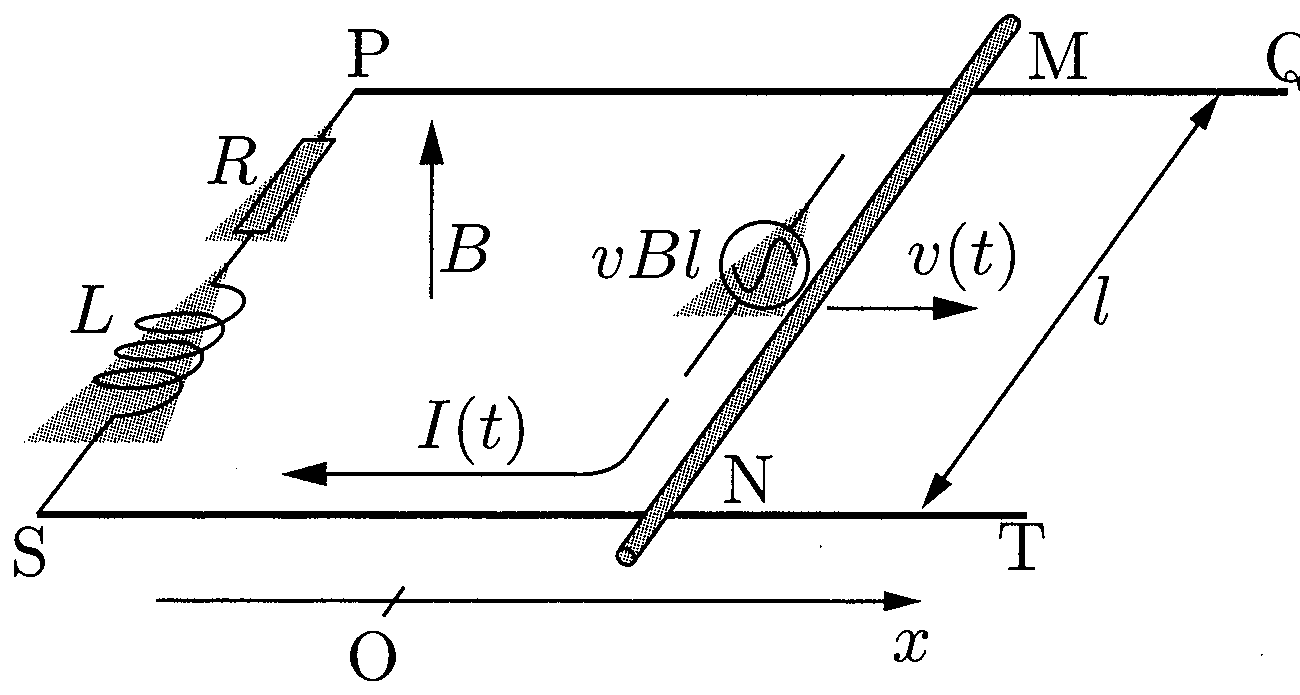
\includegraphics[keepaspectratio,width=50mm]{fig/n32_a130_zu.png}\end{center}
       \begin{center}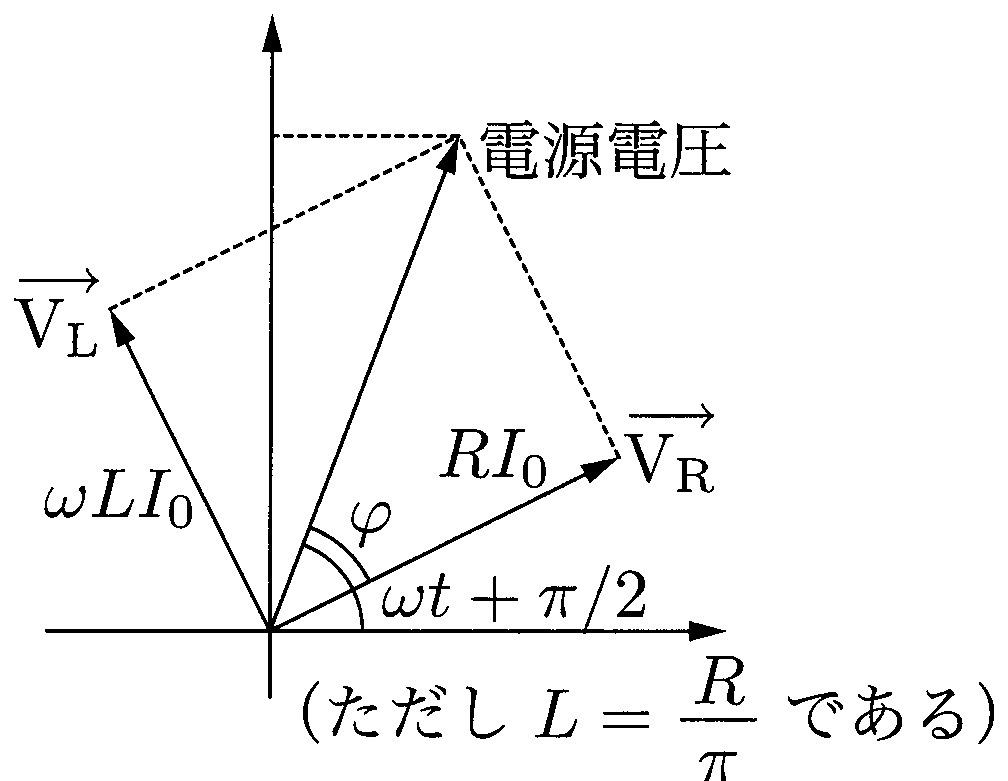
\includegraphics[keepaspectratio,width=46mm]{fig/n32_a130_vec.png}\end{center}
       三平方の定理より$(\omega LI_0)^2+(RI_0)^2=(Bla\omega)^2$なので$I_0=\dfrac{Bla\omega}{\sqrt{2}R}$．また$\tan\varphi=\dfrac{\omega L}{R}=1$より$\varphi=\dfrac{\pi}{4}$．よって
       \[I(t)=\frac{Bla\omega}{\sqrt{2}R}\sin\Bigl(\omega t+\frac{\pi}{4}\Bigr)\U{A}\Ans\]
\ko{3} $\mathrm{M}\to\mathrm{N}$の向きに電流$I(t)$が流れているとき，導体棒は$-x$向きに大きさ$I(t)Bl$の電磁力を受ける．運動方程式は
       \[m\frac{d^2x}{dt^2}=F(t)-I(t)Bl\]
       $\dfrac{d^2x}{dt^2}=\dfrac{dv}{dt}=-a\omega^2\sin\omega t$であるから
       \[\begin{aligned}
         F(t)=&-ma\omega^2\sin\omega t\\
         &+\frac{B^2l^2a\omega}{\sqrt{2}R}\sin\Bigl(\omega t+\frac{\pi}{4}\Bigr)\U{N}
       \end{aligned}\Ans\]
\end{komon}

\MonN{131}{リサジュー図形}\par\nopagebreak
\begin{sisin}
オシロスコープの原理に関する問題で，ブラウン管の知識に加えて交流回路についてもしっかり理解していることが要求される難問である（32.5 の参考）．
極板に電圧$V_x$，$V_y$をかけると，電子ビームは電圧に比例した座標$(x,y)=(\alpha V_x,\alpha V_y)$に輝点を生じる（$\alpha$は装置で決まる定数．第29回の例題26 の電場偏向を参照）．
例えば$x$方向に$V_x=V_0\sin\omega t$をかけると輝点は$x$軸上を往復し，直線が光って見える．さらに$y$方向に同位相の$V_0\sin\omega t$をかけると$y=x$上の線分が，位相が$\dfrac{\pi}{2}$ずれた$V_0\cos\omega t$をかけると円$x^2+y^2=\alpha^2V_0^2$が光って見える．
\begin{center}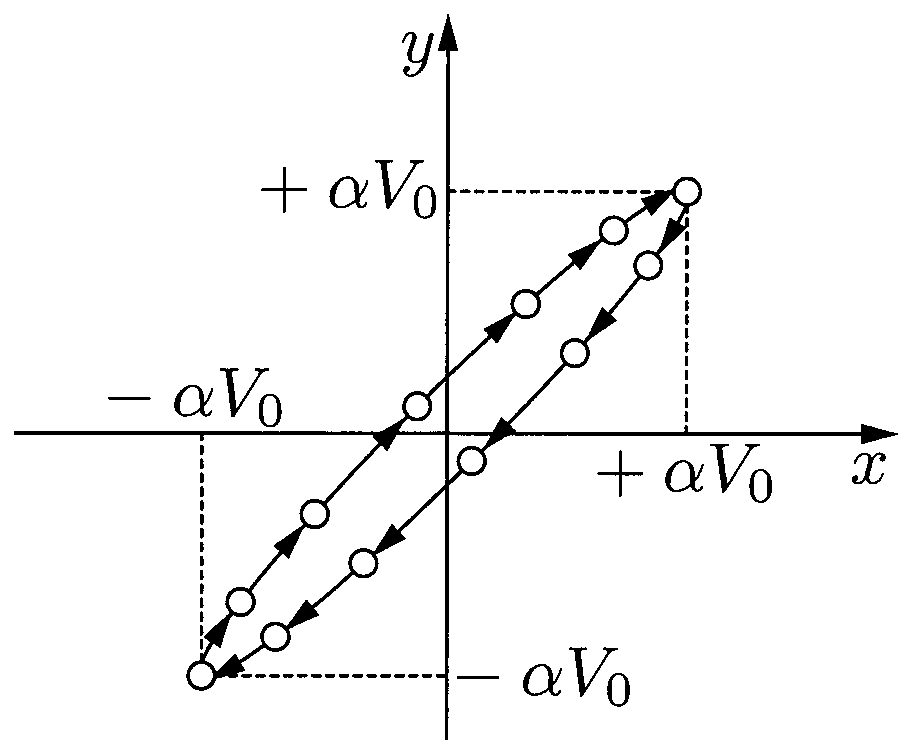
\includegraphics[keepaspectratio,width=38mm]{fig/n32_a131_line.png}\hspace{2mm}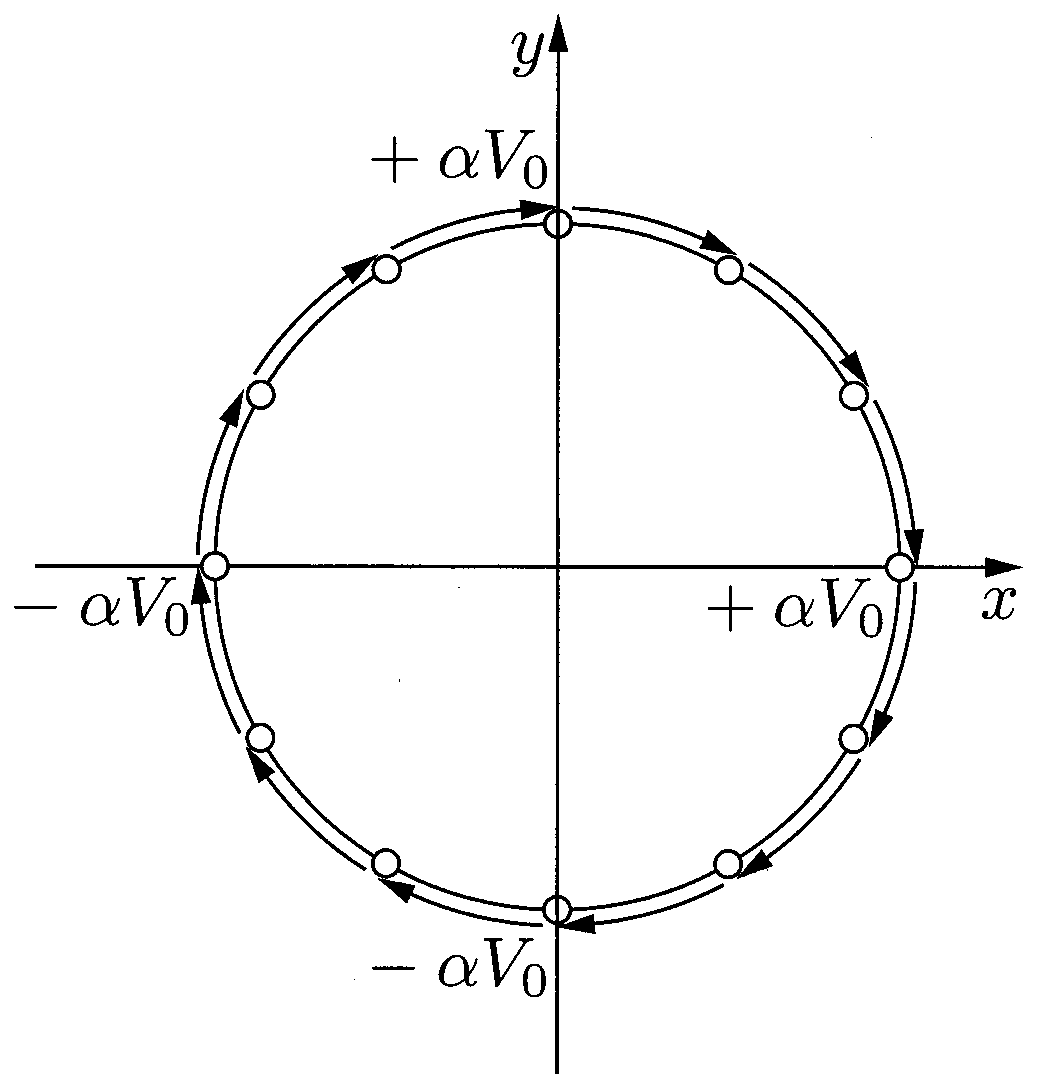
\includegraphics[keepaspectratio,width=38mm]{fig/n32_a131_circ.png}\end{center}
このように，スクリーン上には入力電圧の大きさと位相差によって決まる図形（リサジュー図形）が現れる．
\end{sisin}
\KaiHead
$\overline{\mathrm{X}}$に対して$\mathrm{X}$が高電位のとき電子線は$+x$方向に，$\overline{\mathrm{Y}}$に対して$\mathrm{Y}$が高電位のとき$+y$方向に曲げられるので，輝点は$(x,y)=(\beta V_x,\beta V_y)$に現れる（$\beta$は比例定数）．
図1の回路で$\mathrm{R}$，$\mathrm{L}$に上から下向きに流れる電流を$I(t)=I_0\sin\omega t$とすると
\[V_{\mathrm{AB}}(t)=RI_0\sin\omega t,\quad V_{\mathrm{BC}}(t)=\omega LI_0\cos\omega t\]
であり，$I_0=\dfrac{V_0}{\sqrt{R^2+\omega^2L^2}}$である．

$\mathrm{X}$に$\mathrm{A}$を，$\overline{\mathrm{X}}$に$\mathrm{B}$をつなぎ，$\mathrm{Y}$，$\overline{\mathrm{Y}}$を接地すると，到達点は$(\beta RI_0\sin\omega t,0)$で，$\pm\beta RI_0$の範囲が光る．題意よりこれが$-a\leqq x\leqq a$なので$\beta RI_0=a$，すなわち$\beta=\dfrac{a}{RI_0}$である．
\begin{komon}
\ko{1} 到達点は$(\beta\omega LI_0\cos\omega t,\ 0)$で，$\beta\omega LI_0=\dfrac{\omega L}{R}a$なので
       \[-\frac{2\pi fL}{R}a\leqq x\leqq\frac{2\pi fL}{R}a,\quad y=0\]
       の直線が光って見える．\Ans
\ko{2} 到達点は$(x,y)=(\beta RI_0\sin\omega t,\ \beta\omega LI_0\cos\omega t)$．$t$を消去すると
       \[\frac{x^2}{(\beta RI_0)^2}+\frac{y^2}{(\beta\omega LI_0)^2}=1\]
       の楕円上を高速で動くので，楕円
       \[\frac{x^2}{a^2}+\frac{y^2}{\Bigl(\dfrac{2\pi fL}{R}a\Bigr)^2}=1\ \text{が光って見える．}\Ans\]
\ko{3} (2)で$f$を$\dfrac{1}{3}f$に取り替えればよいので
       \[\frac{x^2}{a^2}+\frac{y^2}{\Bigl(\dfrac{2\pi fL}{3R}a\Bigr)^2}=1\]
       すなわち，(2)の図形が{\gtfamily $y$軸方向に$\dfrac{1}{3}$倍に圧縮された楕円}が現れる．\Ans
\end{komon}

\end{multicols}
